\documentclass[handout,compress]{beamer}

\usetheme[block=fill]{metropolis}

\usepackage{graphicx} % Allows including images
\usepackage{amsmath,amsfonts,amsthm,amssymb}
\usepackage{color}
\usepackage{xcolor,cancel}
%\setitemize{label=\usebeamerfont*{itemize item}%
%	\usebeamercolor[fg]{itemize item}
%	\usebeamertemplate{itemize item}}
\definecolor{mDarkBrown}{HTML}{604c38}
\definecolor{mDarkTeal}{HTML}{23373b}
\definecolor{mLightBrown}{HTML}{EB811B}
\definecolor{mMediumBrown}{HTML}{C87A2F}
\definecolor{mygreen}{HTML}{98C2B9}
\definecolor{myyellow}{HTML}{DFD79C}
\definecolor{myblue}{HTML}{8CA7CC}
\definecolor{kern}{HTML}{8CC2B7}

\usepackage{float}
\usepackage{framed}
\usepackage{epsfig}
\usepackage{graphicx}
\usepackage{subcaption}
\usepackage{ulem}
\usepackage{hhline}
\usepackage{multirow}
\usepackage{comment}   
\usepackage{bbm}
\usepackage{tikz}   
\usepackage{ulem}
\def\Put(#1,#2)#3{\leavevmode\makebox(0,0){\put(#1,#2){#3}}}
\newcommand*\mystrut[1]{\vrule width0pt height0pt depth#1\relax}
\newcommand{\eqdef}{\mathbin{\stackrel{\rm def}{=}}}


\newcommand{\bs}[1]{\boldsymbol{#1}}
\newcommand{\bv}[1]{\mathbf{#1}}
\newcommand{\R}{\mathbb{R}}
\newcommand{\E}{\mathbb{E}}

\DeclareMathOperator*{\argmin}{arg\,min}
\DeclareMathOperator*{\argmax}{arg\,max}
\DeclareMathOperator{\nnz}{nnz}
\DeclareMathOperator{\Var}{Var}
\DeclareMathOperator{\sinc}{sinc}
\DeclareMathOperator{\mv}{mv}
\DeclareMathOperator{\sgn}{sgn}
\DeclareMathOperator{\step}{step}
\DeclareMathOperator{\gap}{gap}
\DeclareMathOperator{\poly}{poly}
\DeclareMathOperator{\tr}{tr}
\DeclareMathOperator{\orth}{orth}
\newcommand{\norm}[1]{\|#1\|}
\captionsetup[subfigure]{labelformat=empty}
\captionsetup[figure]{labelformat=empty}
\DeclareMathOperator*{\lmin}{\lambda_{min}}
\DeclareMathOperator*{\lmax}{\lambda_{max}}

\newcommand{\specialcell}[2][c]{%
	\begin{tabular}[#1]{@{}c@{}}#2\end{tabular}}
\newcommand{\specialcellleft}[2][c]{%
	\begin{tabular}[#1]{@{}l@{}}#2\end{tabular}
}

\usepackage{tabstackengine}
\stackMath

\newtheorem{claim}[theorem]{Claim}


%----------------------------------------------------------------------------------------
%	TITLE PAGE
%----------------------------------------------------------------------------------------

\title{CS-UY 4563: Lecture 23 \\ Semantic Embeddings, Clustering}
\author{NYU Tandon School of Engineering, Prof. Christopher Musco}
\date{}

\begin{document}
	
	\begin{frame}
		\titlepage 
	\end{frame}
	
	\metroset{titleformat=smallcaps}
	


\begin{frame}
	\frametitle{course logistics}
	If you have not already, \textbf{sign up for a time slot to present your project}. 5 Minute slots on Wed. 5/6 and Mon. 5/11.
	\begin{itemize}
		\item Prepare slides with images to showcase your project. 
		\item Presentation followed by a few questions. 
		\item  What's the problem you are looking at? Why's it interesting and exciting? 
		\item  What data are you using? What features? What approaches have you tried, what stumbling blocks have you hit?
	\end{itemize}

\begin{center}
\textbf{\alert{Presentation will count towards final project grade.}}
\end{center}
\end{frame}

\begin{frame}
	\frametitle{4 page final report}
	\small
	This project is about \emph{exploring a data set}. Report should be a guide through that exploration process. 
	\begin{itemize}
		\item Explain the data set in detail. Show us what the data looks like with examples, scatter plots, histograms, etc. 
		\item What's the question you sought to answer? What features did you focus on to answer that question and why?
		\item If you method worked, how well did it work? How did you evaluate it? What examples did it do well on? Where did it fail? How would that guide future work?
		\item If you had some setbacks, why? How did you try to address them? Don't include \emph{every failure} but discuss any interesting ones.
	\end{itemize}
\begin{center}
	\textbf{\alert{Think about what you might include if you were building a student lab for your project data.}}
\end{center}
\end{frame}

\begin{frame}
	\frametitle{4 page final report}
	What I'm looking for:
	\begin{itemize}
		\item \textbf{Used appropriate tools from the class:} E.g. feature selection or regularization if you over fit, train-test split to evaluate models and set hyper-parameters, etc.
		\item \textbf{Good baseline exploration:} Most common class, $k$-nn, linear regression, etc.
		\item \textbf{Well justified choices:} Loss functions that make sense, final performance metrics that make sense, logical feature transformations. 
		\item \textbf{Creativity:} \emph{Most} ideas (for feature transformations, new models, etc.) will not pan out. But I want to see that you adapted your approach to what you saw in the data. 
	\end{itemize}
	
\end{frame}


%\begin{itemize}
%	\item What's the problem you are looking at? 
%	\item Why is it an interesting? Why is it suitable to a machine learning approach?
%	\item What data are you using? What features?
%	\item What approaches have you tried, what stumbling blocks have you hit?
%\end{itemize}


\begin{frame}
	\frametitle{principal component analysis}
	\textbf{Recall:} Given input $\bv{X} \in \R^{n\times d}$ and target rank $k$, find $\bv{W}_1$, $\bv{W}_2$ too minimize $\|X - \bv{W}_1\bv{W}_2 \|_F^2$
		\begin{center}
		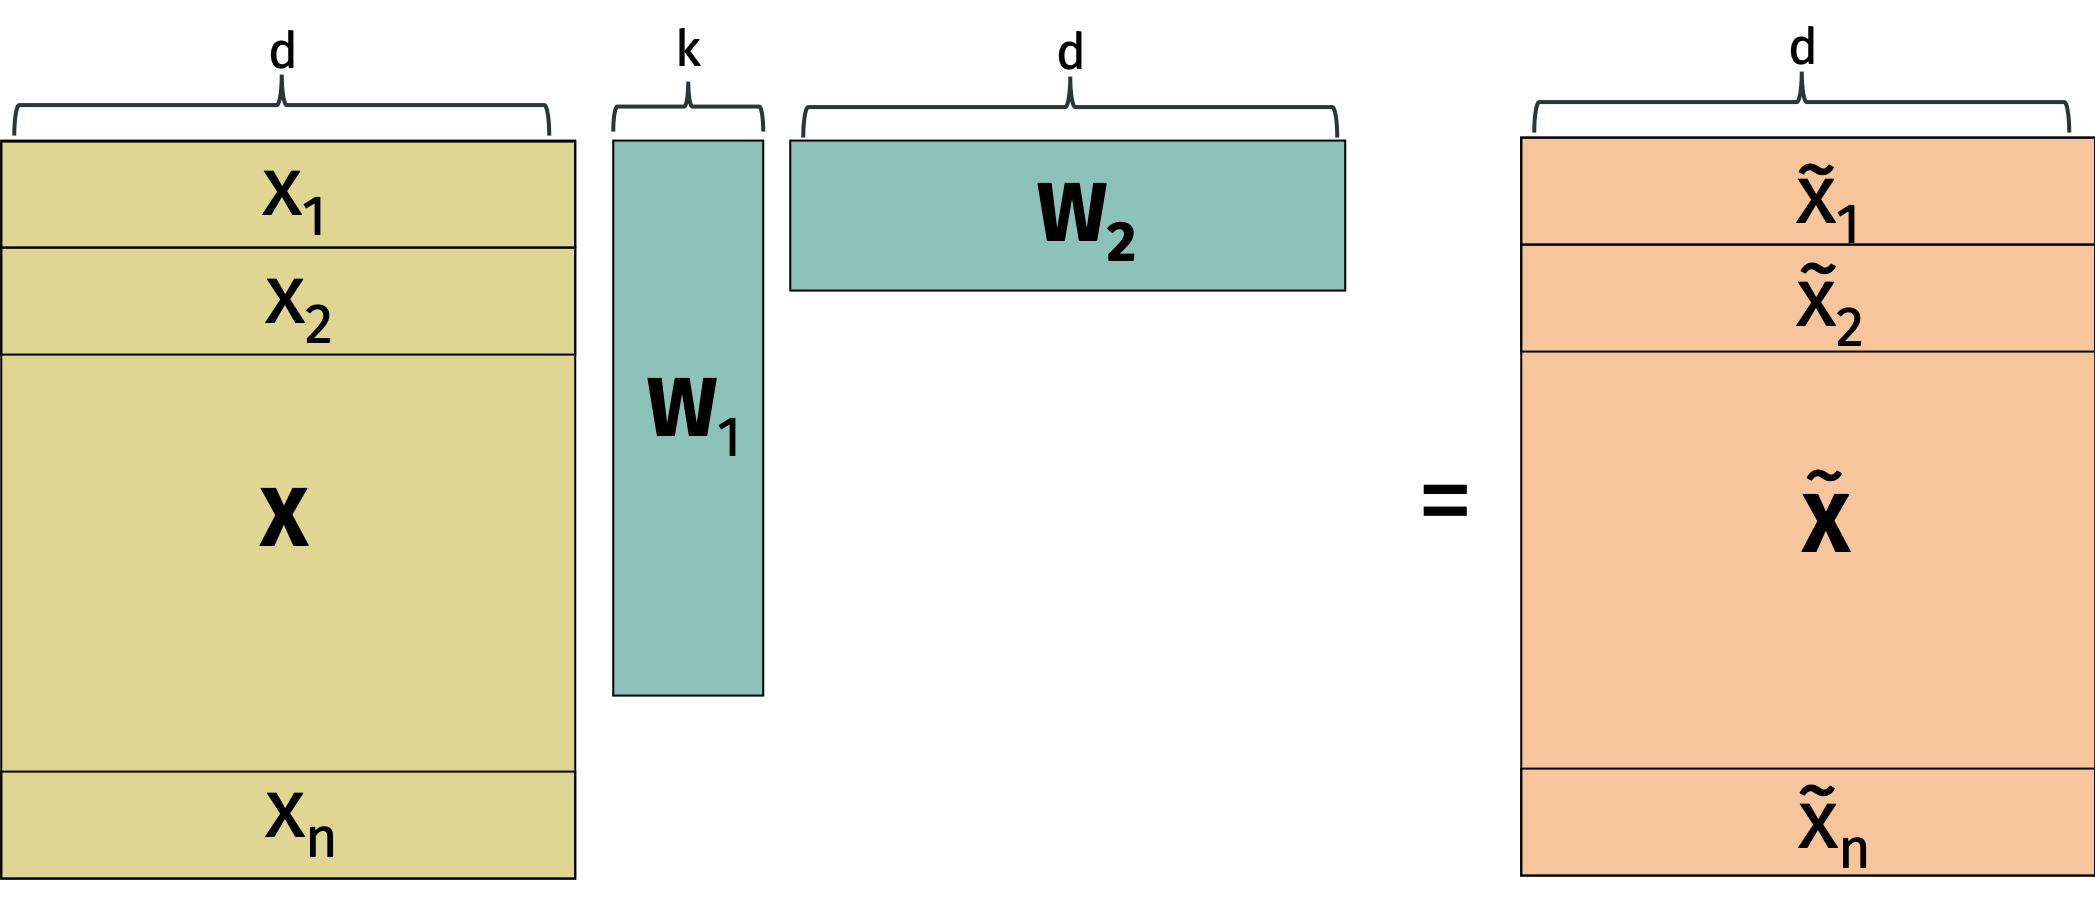
\includegraphics[width=.8\textwidth]{low_rank_basic.png}.
	\end{center}
This problem can be solved efficiently using the \emph{singular value decomposition} of $\bv{X}$. 
\end{frame}

\begin{frame}
	\frametitle{singular value decomposition}
	\small
	\emph{Any} matrix $\bv{X}$ can be decomposed as:
	\begin{center}
		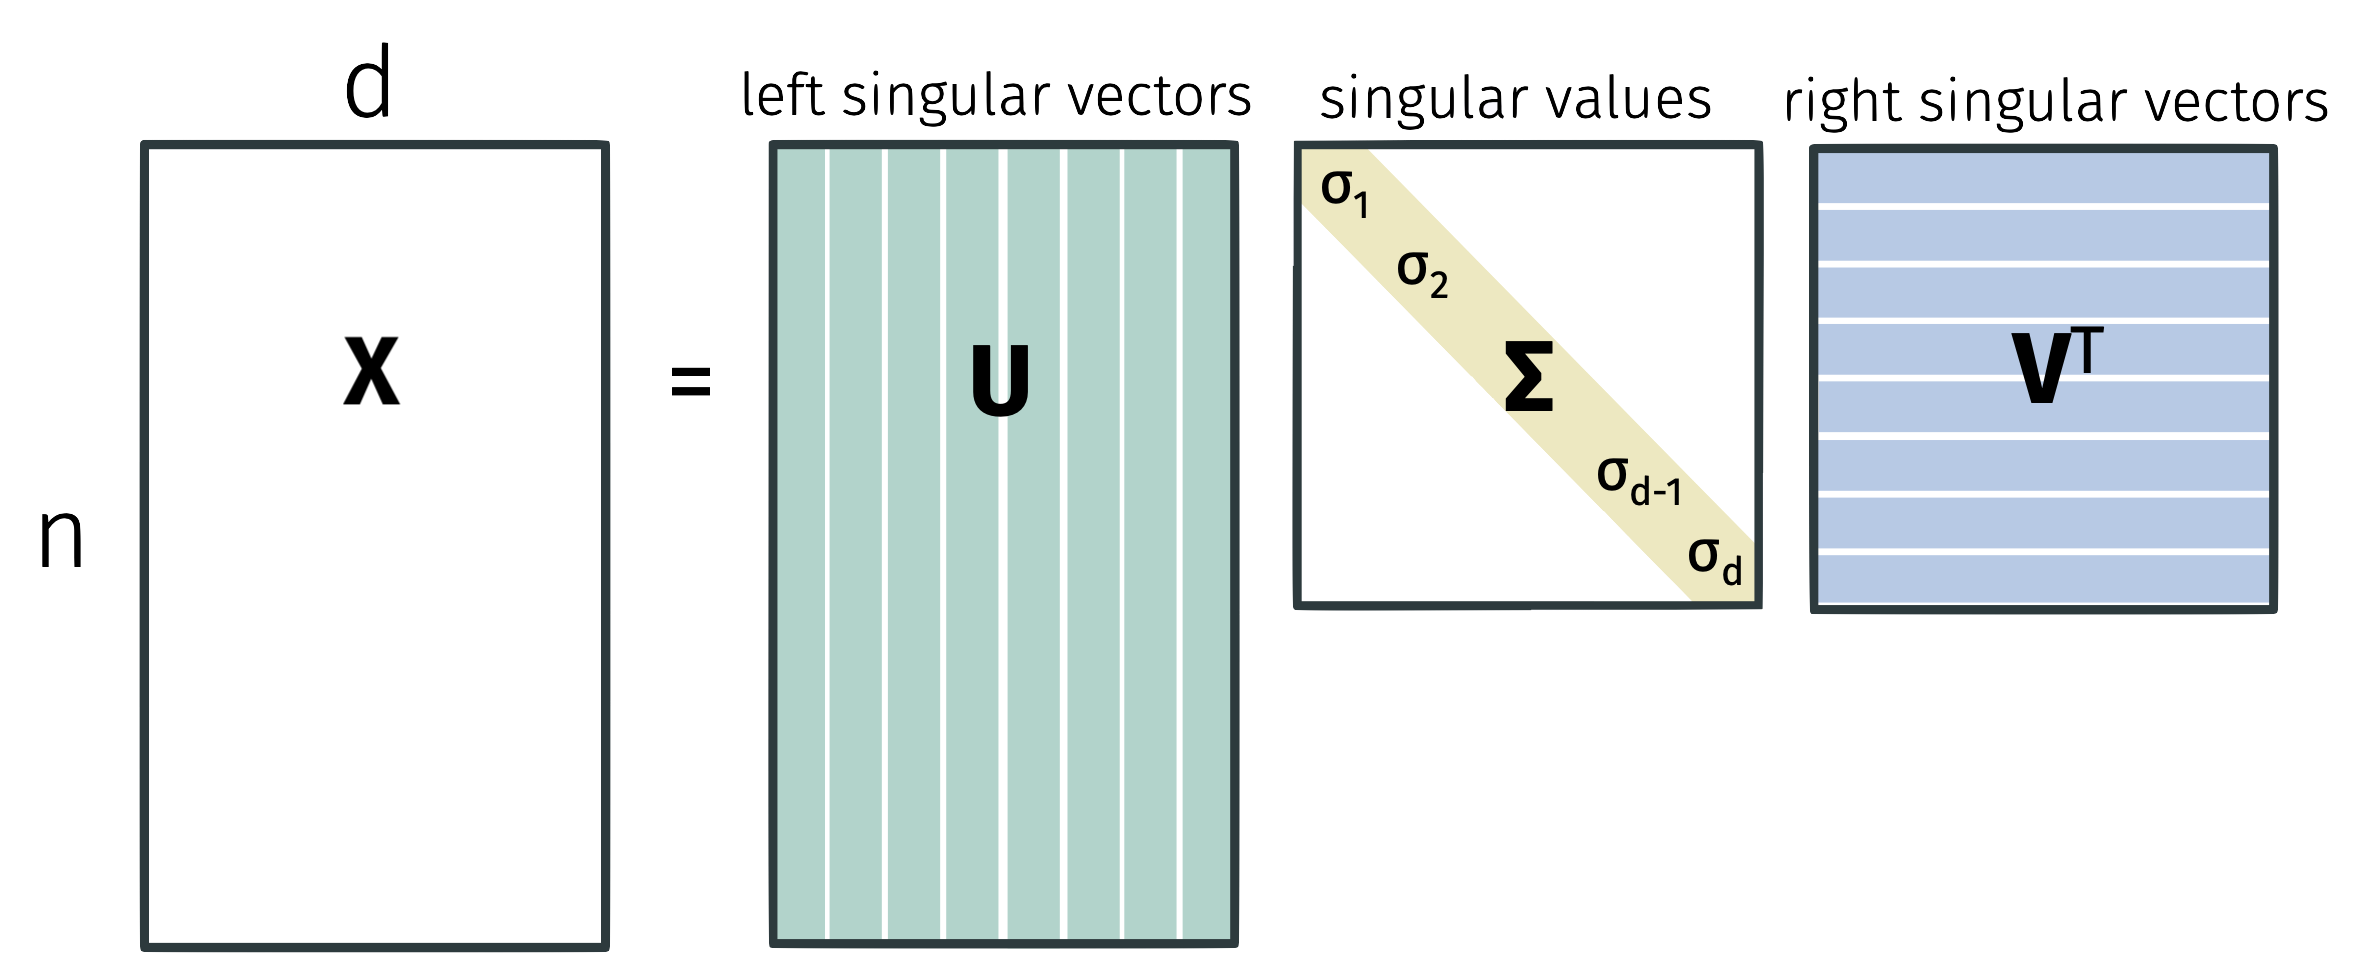
\includegraphics[width=.9\textwidth]{svd.png}
	\end{center} 
	Where $\bv{U}^T\bv{U} = \bv{I}$,  $\bv{V}^T\bv{V} = \bv{I}$, and $\sigma_1 \geq \sigma_2 \geq \ldots \sigma_d \geq 0$. I.e. $\bv{U}$ and $\bv{V}$ are \emph{orthogonal matrices}.
\end{frame}

\begin{frame}[t]
	\frametitle{connection to eigendecomposition}
	Recall that for a matrix $\bv{M}\in \R^{p\times p}$, $\bv{q}$ is an \emph{eigenvector} of $\bv{M}$ if $\lambda \bv{q} = \bv{M}\bv{q}$ for any scalar $\lambda$. 
	\begin{itemize}
		\item $\bv{U}$'s columns (the left singular vectors) are the orthonormal eigenvectors of $\bv{X}\bv{X}^T$. 
		\item $\bv{V}$'s columns (the right singular vectors) are the orthonormal eigenvectors of $\bv{X}^T\bv{X}$. 
		\item $\sigma_i^2 = \lambda_i(\bv{X}\bv{X}^T) = \lambda_i(\bv{X}^T\bv{X})$
	\end{itemize}
Easy to check directly. This means you can use any (symmetric) eigensolver for computing the SVD. 
\end{frame}

\begin{frame}[t]
	\frametitle{singular value decomposition}
	\small
	\texttt{U,S,V = scipy.sparse.linalg.svds(X, k).} 
	\begin{center}
		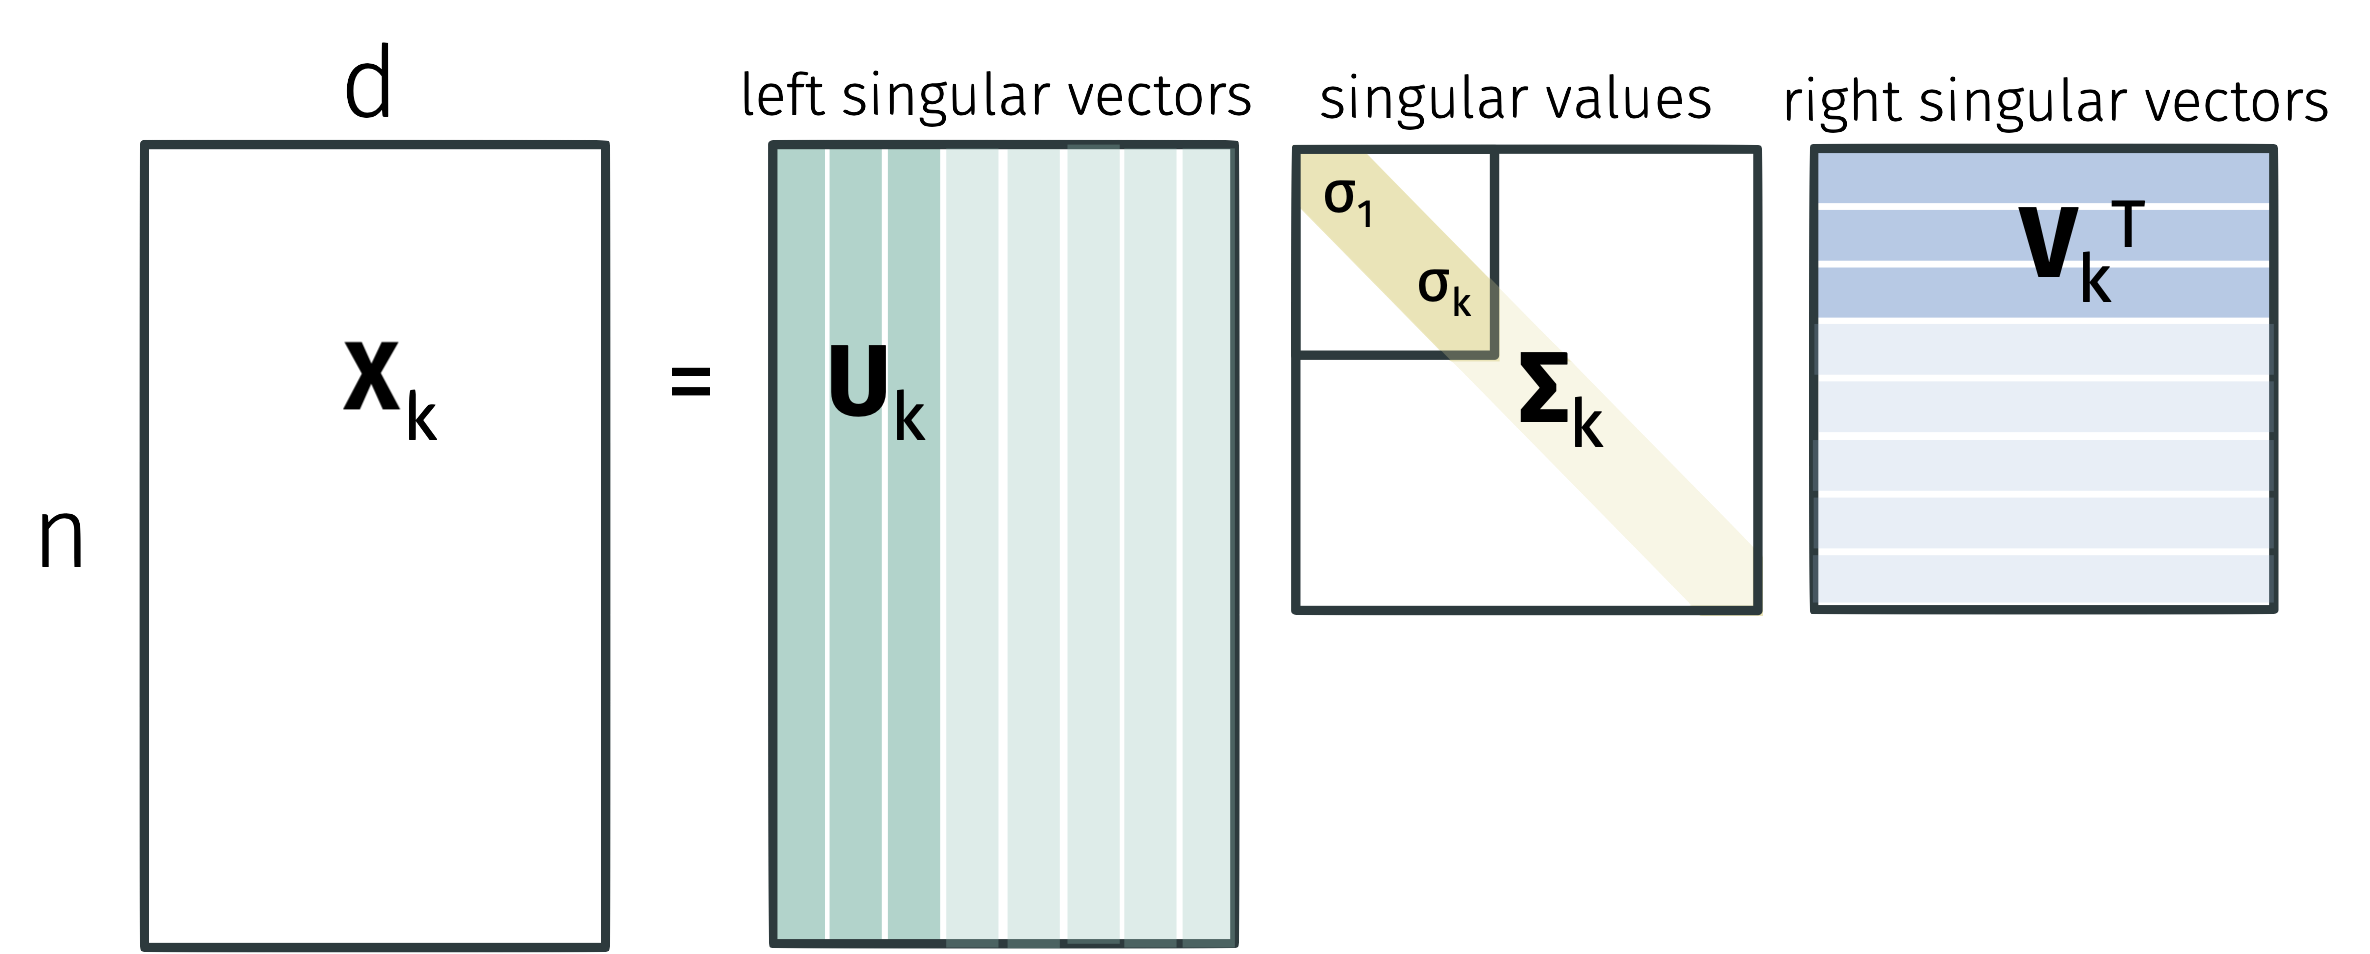
\includegraphics[width=.9\textwidth]{svdk.png}
	\end{center} 
	\textbf{Eckart–Young–Mirsky Theorem:} For any $k \leq d$, $\bv{X}_k = \bv{U}_k\bs{\Sigma}_k\bv{V}_k^T = \bv{X}\bv{V}_k\bv{V}_k^T $ is the optimal $k$ rank approximation to $\bv{X}$:
	\begin{align*}
	\bv{X}_k = 	\argmin_{\tilde{\bv{X}} \text{ with rank $\leq k$} } \|\bv{X} - \tilde{\bv{X}}\|_F^2.
	\end{align*}
	
	For PCA, set $\bv{W}_1 = \bv{V}_k$, $\bv{W}_1 = \bv{V}_k^T$.
\end{frame}

\begin{frame}[t]
	\frametitle{principal component analysis}
	\begin{center}
		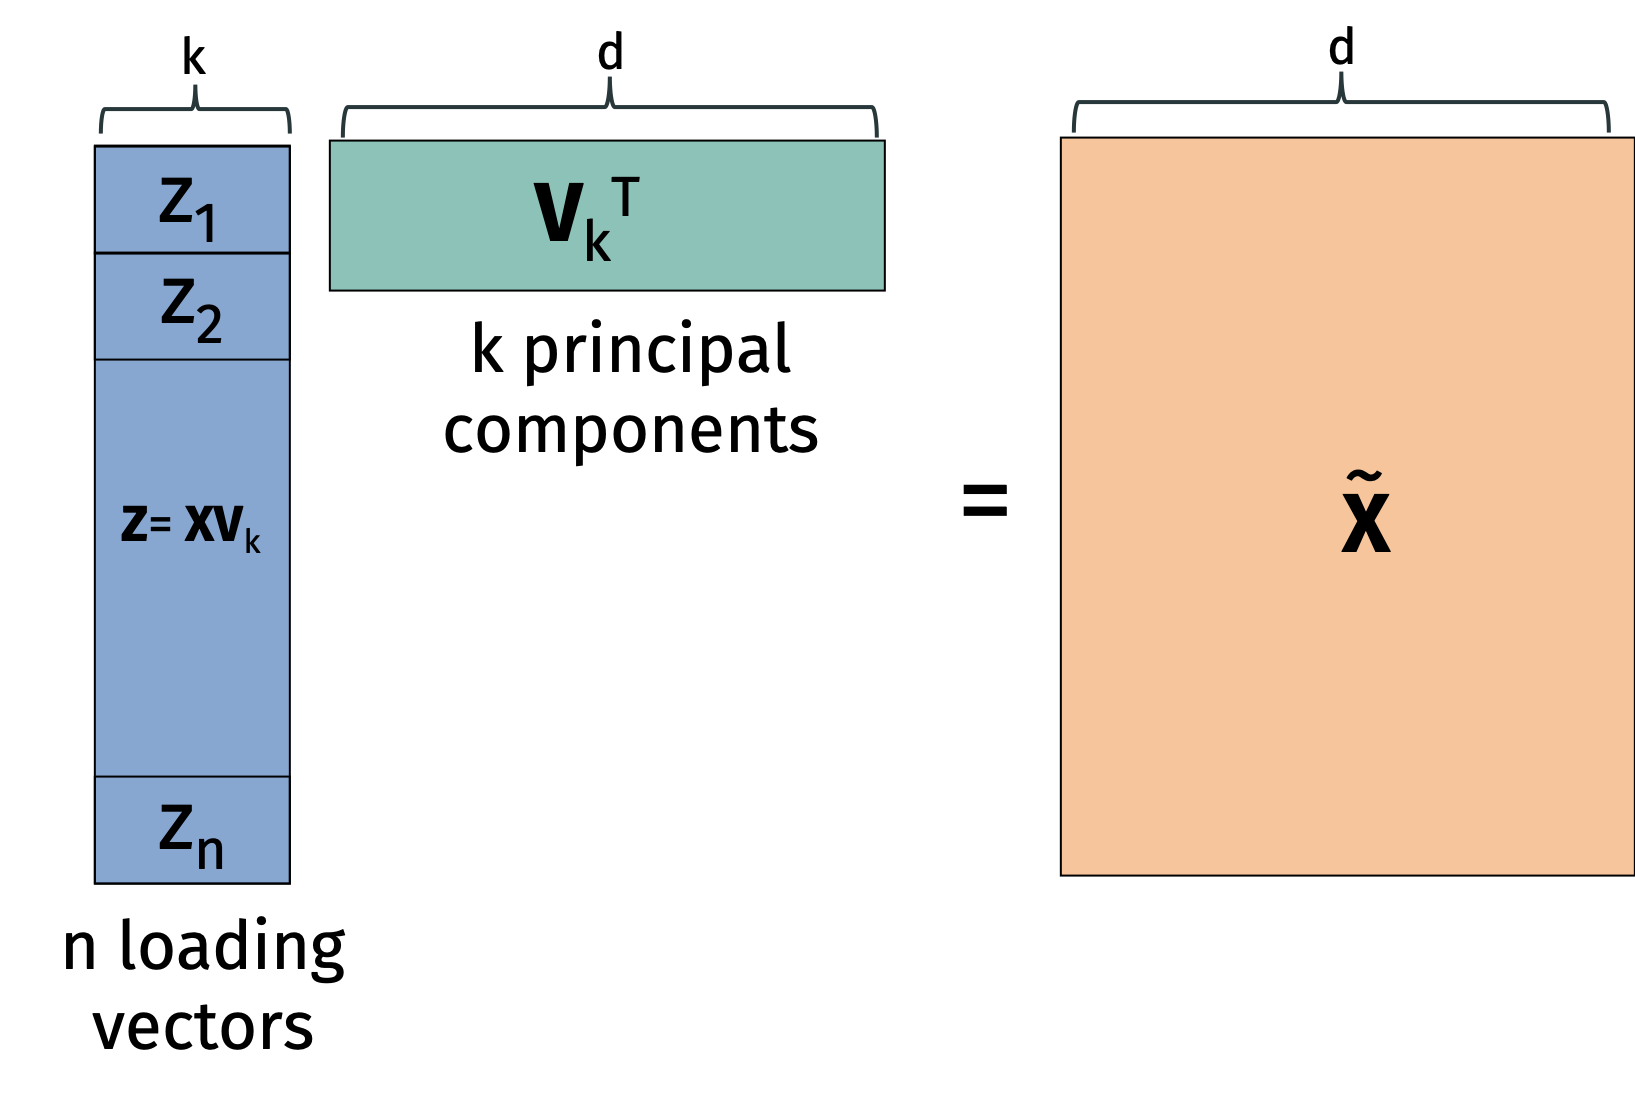
\includegraphics[width=.8\textwidth]{pca.png}
	\end{center} 
Usually $\vec{X}$'s columns (features) are mean centered and normalized to variance $1$ before computing principal components.
\end{frame}

\begin{frame}
	\frametitle{pca applications}
	\textbf{Like any autoencoder, PCA can be used for:}
	\begin{itemize}
		\item Feature extraction
		\item Denoising and rectification
		\item Data generation
		\item Compression
		\item Visualization
	\end{itemize}
\begin{center}
	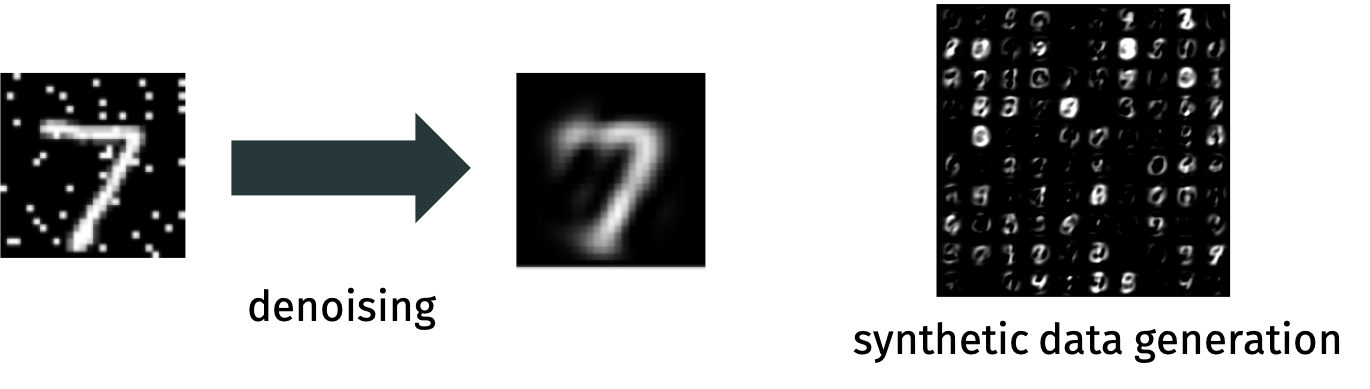
\includegraphics[width=.8\textwidth]{pca_applications.png}
\end{center}
\end{frame}

\begin{frame}[t]
	\frametitle{low-rank approximation}

\begin{center}
	\vspace{-.5em}
	The larger we set $k$, the better approximation we get.
	
	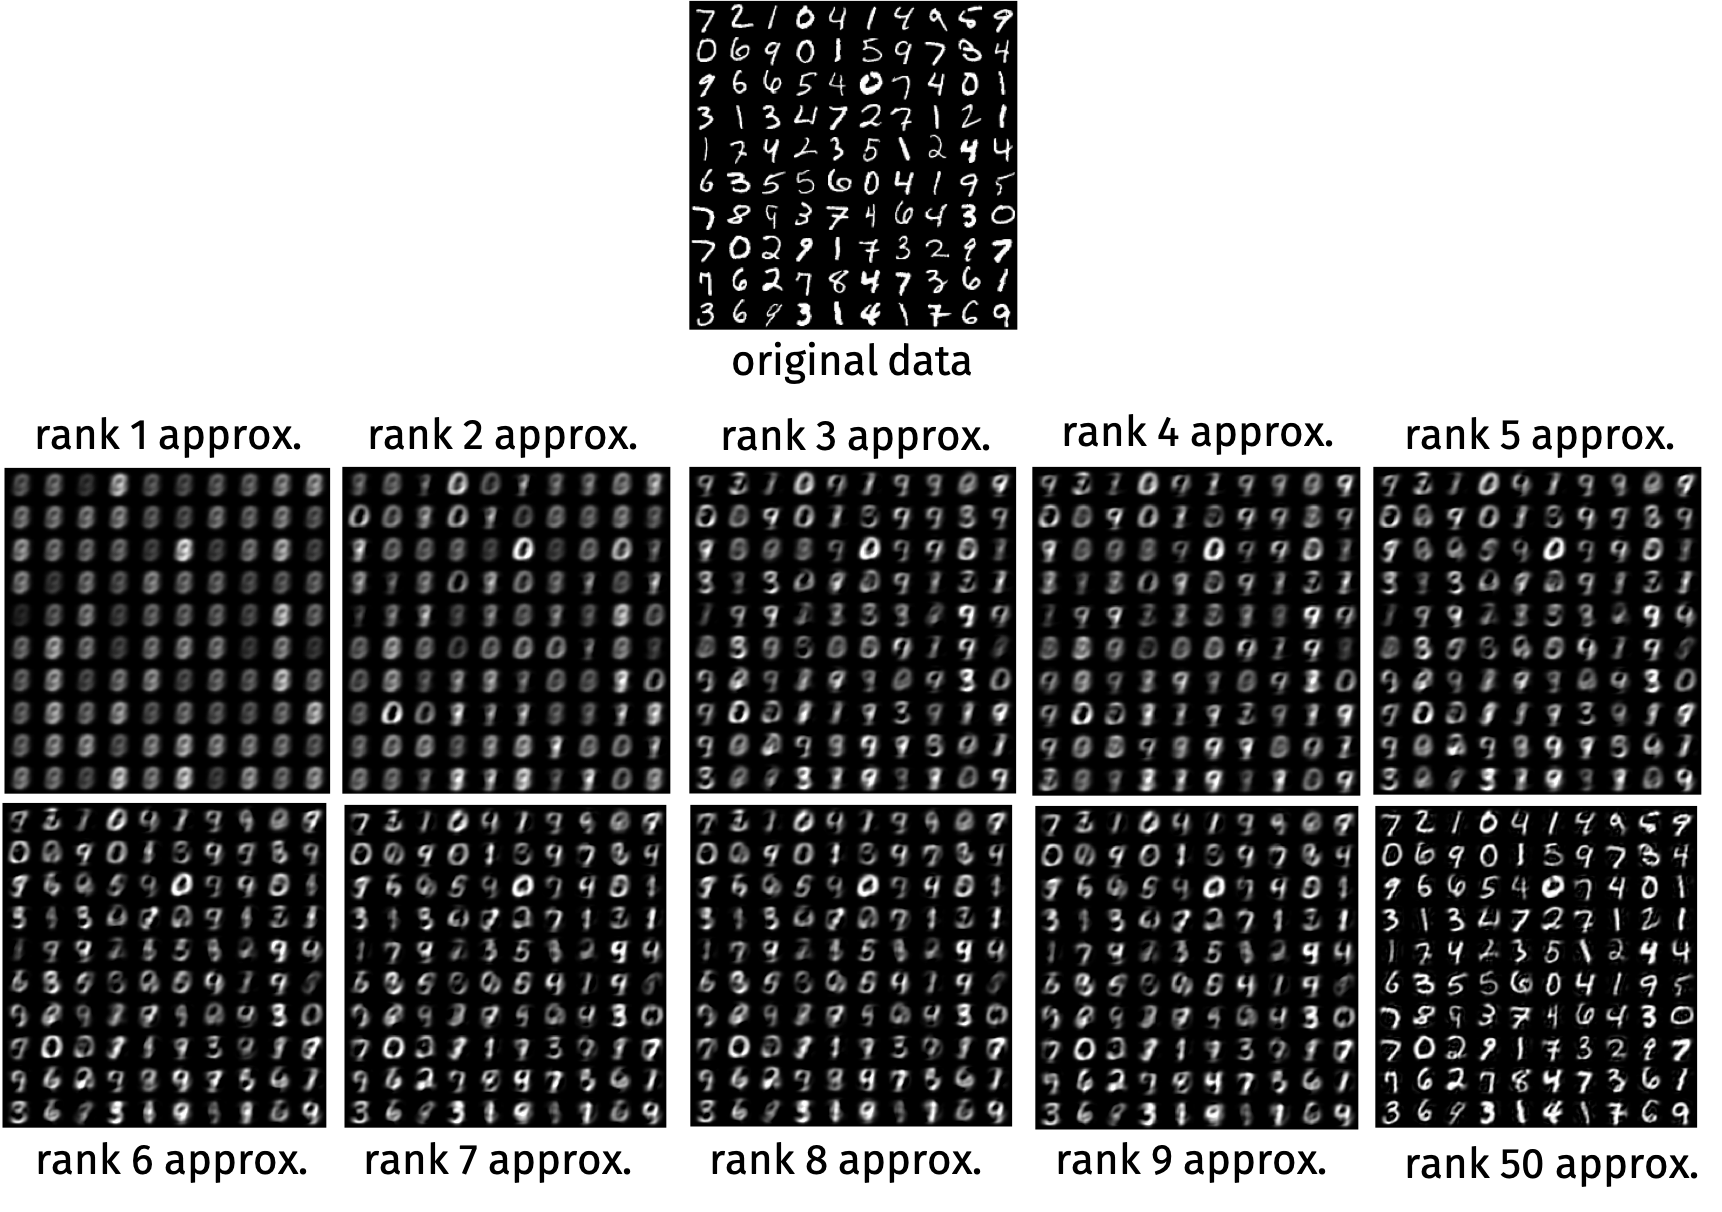
\includegraphics[width=.95\textwidth]{low_rank_approxs2.png}
	\end{center}
\end{frame} 

\begin{frame}[t]
	\frametitle{low rank approximation}
	Error vs. $k$ is dictated by $\bv{X}$'s singular values. This is often called the \textbf{spectrum} of $\bv{X}$. 
	\begin{align*}
	\|\bv{X} - \bv{X}_k\|_F^2 = \sum_{i=k}^d \sigma_i^2.
	\end{align*} 
	\begin{center}
		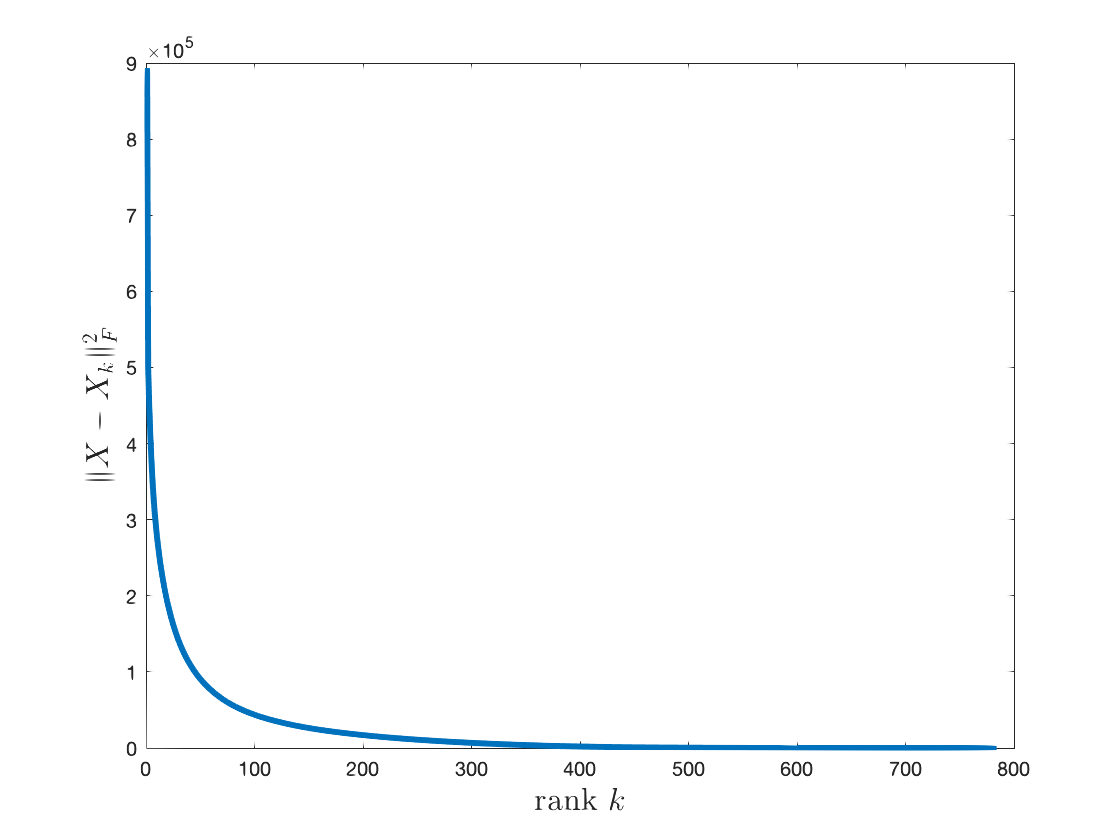
\includegraphics[width=.6\textwidth]{pca_errors.png}
	\end{center}
\end{frame}

\begin{frame}
	\frametitle{low rank intuition}
	Which of these data sets has the better low-rank matrix:
	\begin{enumerate}
		\item  House data: 
		\begin{align*}
		\scriptsize
		\bv{x} = \left[\text{\# bedrooms},  \text{\# bathrooms}, \text{list price}, \text{sale price}, \text{property tax} \right]
		\end{align*}
		
		\item  \normalsize{Student data:}
		\begin{align*}
		\scriptsize
		\bv{x} = \left[\text{gender}, \text{year},  \text{age}, \text{GPA}, \text{engineering major}\right]
		\end{align*}	
	\end{enumerate}
\end{frame}

\begin{frame}
	\frametitle{low rank intuition}
	Which of these data sets has the better low-rank matrix:
	\begin{enumerate}
		\item  House data: 
		\begin{align*}
		\scriptsize
		\bv{x} = \left[\text{\# bedrooms},  \text{\# bathrooms}, \text{list price}, \text{sale price}, \text{property tax} \right]
		\end{align*}
		
		\item  \normalsize{Student data:}
		\begin{align*}
		\scriptsize
		\bv{x} = \left[\text{gender}, \text{year},  \text{age}, \text{GPA}, \text{engineering major}\right]
		\end{align*}	
	\end{enumerate}
\end{frame}

\begin{frame}
	\frametitle{column redundancy}
	\textbf{Colinearity} of data features leads to an approximately low-rank data matrix. 
	\begin{center}
		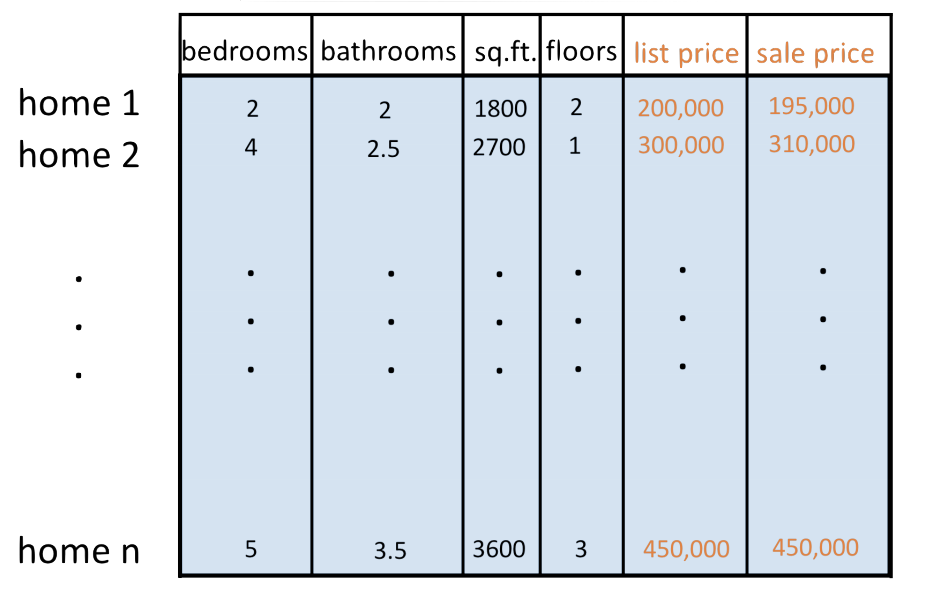
\includegraphics[width=.7\textwidth]{columnview.png}
	\end{center}
$\text{sale price} \approx 1.05 \cdot \text{list price}$. \hspace{5em} $\text{property tax} \approx .01 \cdot \text{list price}$.
\end{frame}


\begin{frame}
	\frametitle{column redundancy}
	Sometimes these relationships are simple, other times more complex. 
	But as long as there exists \emph{linear} relationships between features, we will have a lower rank matrix. 
	
	\begin{align*}
	\textbf{yard size} \approx \textbf{lot size} - \frac{1}{2}\cdot\textbf{square footage}. 
	\end{align*}
	
	\begin{align*}
	\textbf{cumulative GPA} \approx &\frac{1}{4}\cdot\textbf{year 1 GPA} + \frac{1}{4}\cdot\textbf{year 2 GPA} \\ &+ \frac{1}{4}\cdot\textbf{year 3 GPA} + \frac{1}{4}\cdot\textbf{year 4 GPA}.
	\end{align*}
\end{frame}

\begin{frame}
	\frametitle{low-rank intuition}
	Which of these data sets has a good low-rank matrix:
	\begin{enumerate}
		\item  Genetic data: 
		
		\begin{center}
		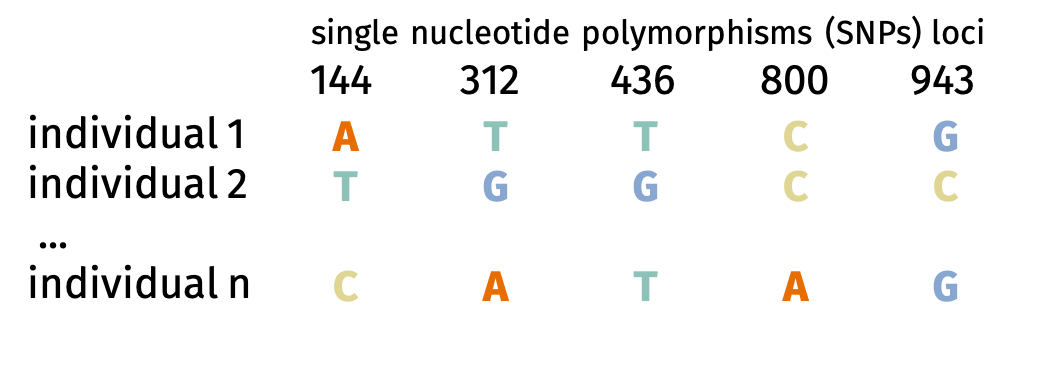
\includegraphics[width=.7\textwidth]{dna_data.png}
		\end{center}
		
		\item ``Term-document'' matrix with bag-of-words data:
		
		\begin{center}
			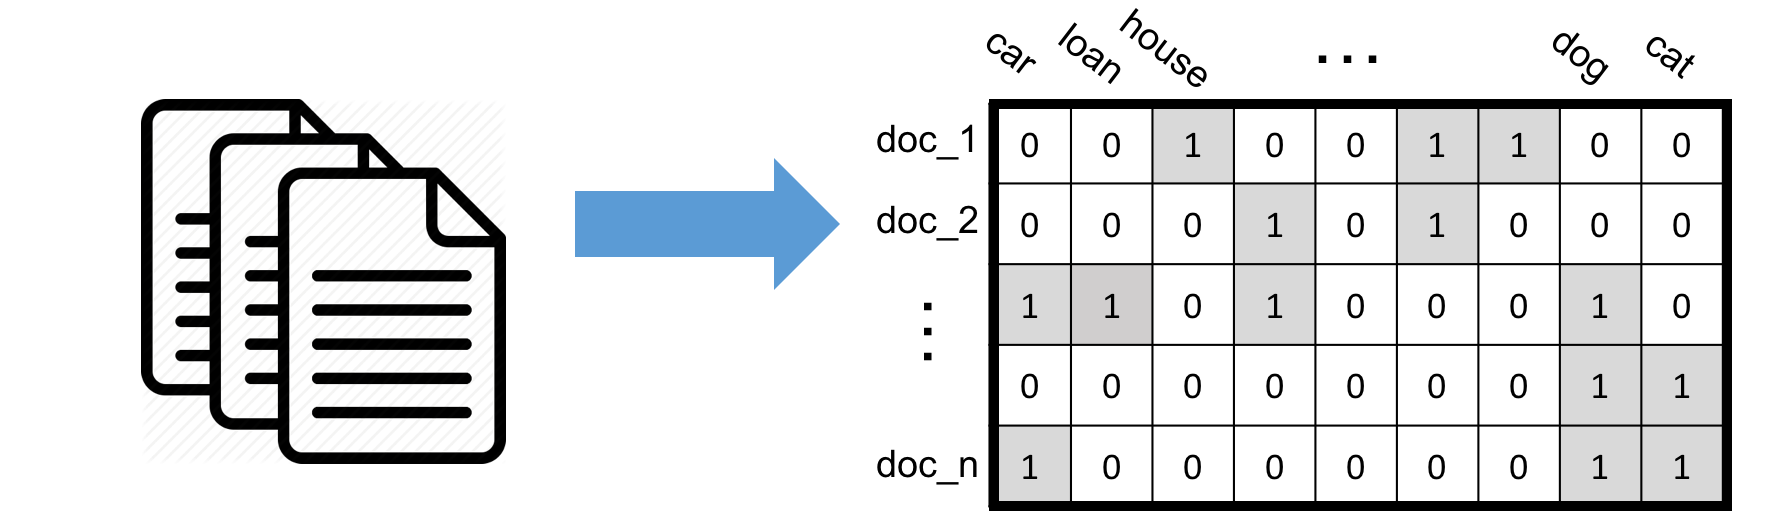
\includegraphics[width=.7\textwidth]{term_doc.png}
		\end{center}
	\end{enumerate}
\end{frame}

\begin{frame}
	\frametitle{examples of low-rank structure}
	SNPs matrices tend to be very low-rank.
	\begin{center}
		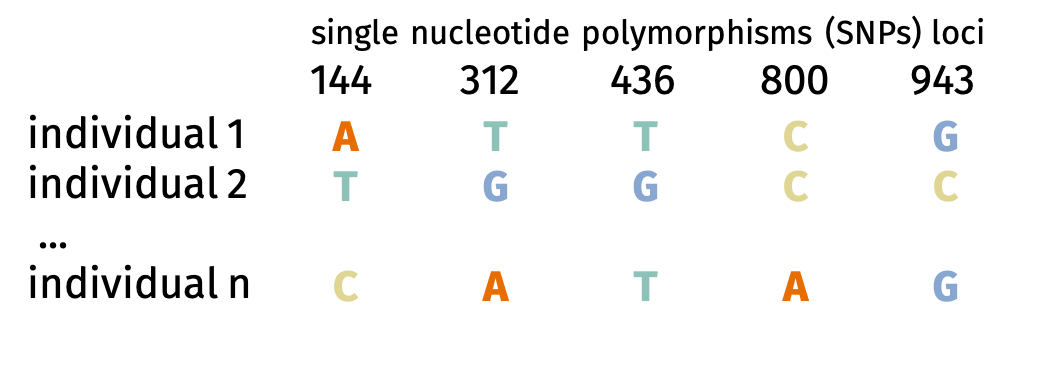
\includegraphics[width=.7\textwidth]{dna_data.png}
	\end{center}
Most of the information in $\vec{x}$ is explained by just a few \textbf{latent variable}. 
	\begin{center}
		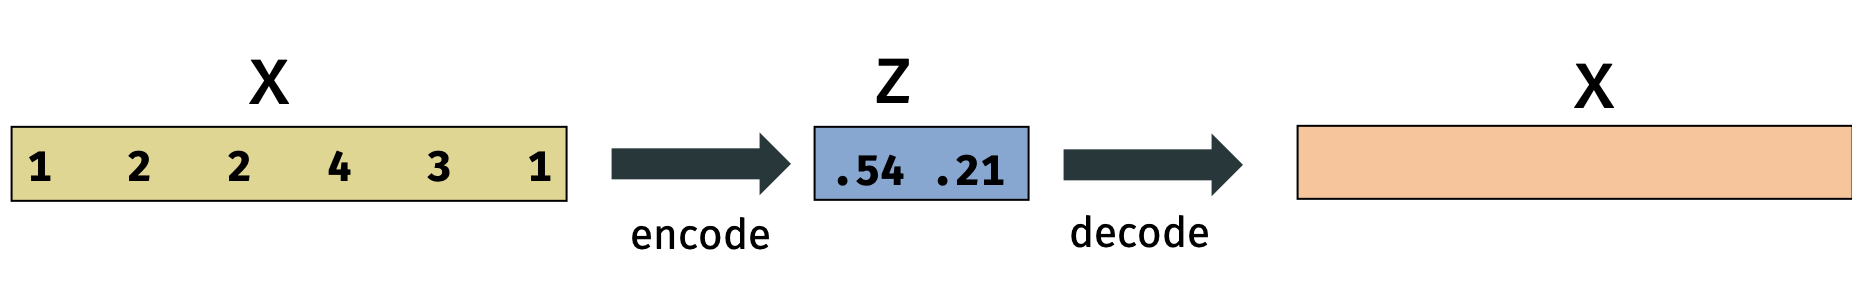
\includegraphics[width=.7\textwidth]{gene_compression.png}
	\end{center}
\end{frame}


\begin{frame}
	\frametitle{similarity preservation}\small
	\textbf{Very important note:} Latent feature vectors preserve similarity and distance information in the original data. 
	
	Let $\vec{x}_1\ldots, \vec{x}_n \in \R^d$ be our original data vectors. $\vec{z}_1\ldots, \vec{z}_n \in\R^k$ be our loading vectors. $\tilde{x}_1\ldots, \tilde{x}_n \in \R^d$ be our low-rank approximated data.
	\begin{enumerate}
		\item If we have a good low-rank approximation, we expect that $\vec{x}_i$ is close to $\tilde{x}_i$ for most $i$. 
		\item So for most $i,j$ pairs, $\langle\vec{x}_i,\vec{x}_j \rangle \approx \langle\tilde{x}_i,\tilde{x}_j \rangle$ and $\|\vec{x}_i - \vec{x}_j\|_2 \approx \|\tilde{x}_i - \tilde{x}_j\|_2$. 
		\item  $\langle\tilde{x}_i,\tilde{x}_j \rangle = \langle\bv{V}_k\vec{z}_i,\bv{V}_k\vec{z}_j \rangle$ since $\bv{V}_k$ is orthogonal. And $\|\tilde{x}_i - \tilde{x}_j\|_2 = \|\bv{V}_k\vec{z}_i - \bv{V}_k\vec{z}_j\|_2$.
	\end{enumerate}
\begin{center}
	\large
	\alert{
	\textbf{Conclusion:} $\langle\vec{x}_i,\vec{x}_j \rangle \approx \langle\vec{z}_i,\vec{z}_j \rangle$ and $\|\vec{x}_i - \vec{x}_j\|_2 \approx \|\vec{z}_i - \vec{z}_j\|_2$.
}
\end{center}

\end{frame}

\begin{frame}
	\frametitle{examples of low-rank structure}
	``Genes Mirror Geography Within Europe'' -- Nature, 2008.
	\begin{center}
		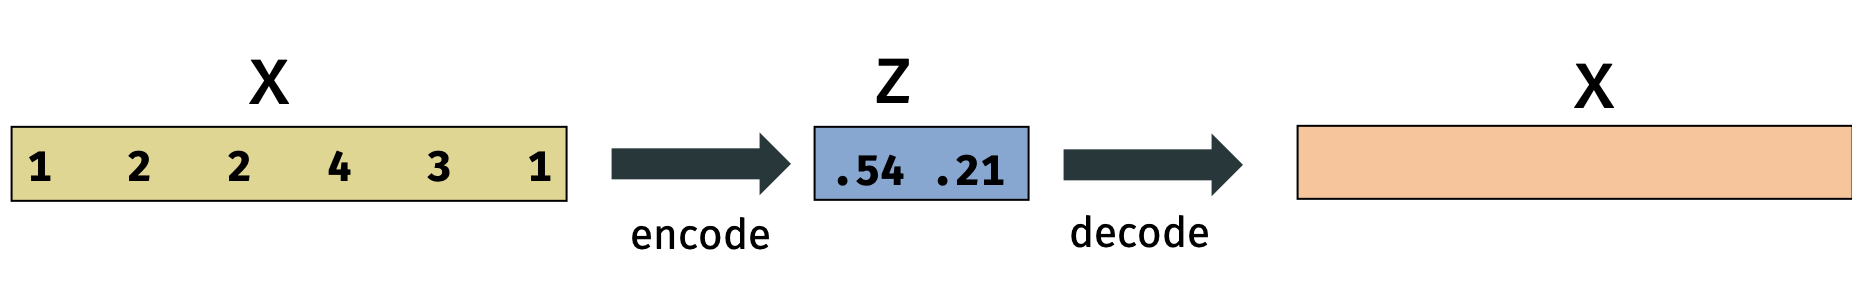
\includegraphics[width=.8\textwidth]{gene_compression.png}
	\end{center}
	In data collected from European populations, latent variables capture information about \emph{geography}. 
\begin{align*}
\vec{z}[1] &\approx \text{relative north-south position of birth place}\\
\vec{z}[2] &\approx \text{relative east-west position of birth place}
\end{align*}
\begin{center}
\textbf{Individuals born in similar places tend to have similar genes.}
\end{center} 
\end{frame}


\begin{frame}
	\frametitle{pca for data visualization}
	``Genes Mirror Geography Within Europe'' -- Nature, 2008.
	\begin{center}
		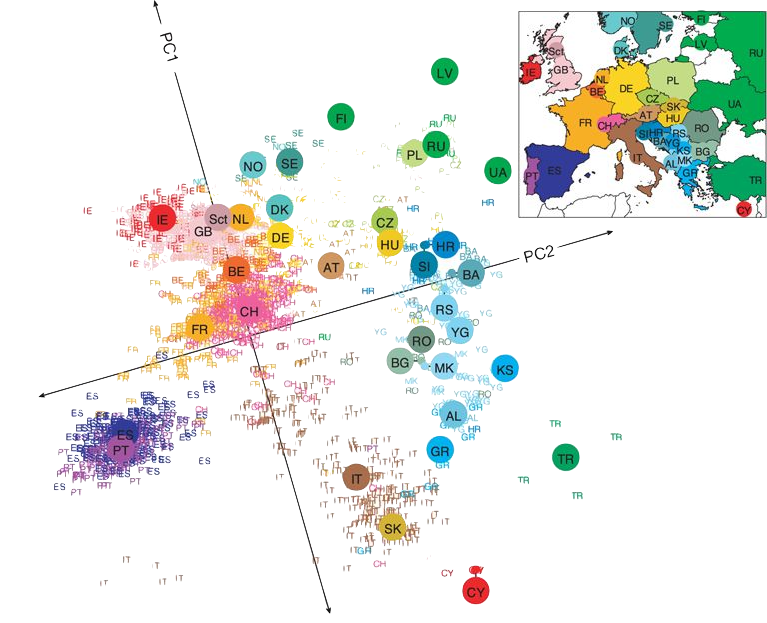
\includegraphics[width=.65\textwidth]{genes_pca.png}
	\end{center}
	Can be easily visualized using PCA! Plot each data example $\vec{x}$ using two loading variables in $\vec{z}$.
\end{frame}

\begin{frame}
	\frametitle{term document matrix}
	Word-document matrices tend to be low rank. 
	\begin{center}
		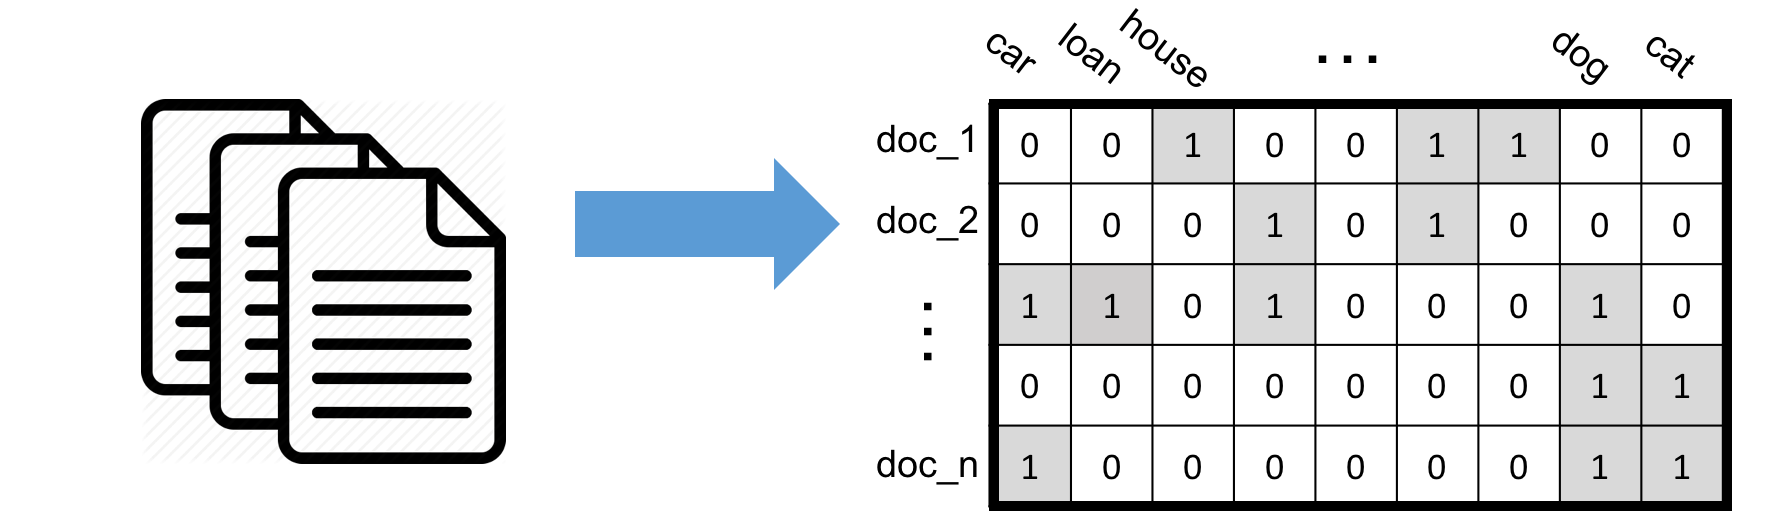
\includegraphics[width=.7\textwidth]{term_doc.png}
	\end{center}
	Documents tend to fall into a relatively small number of different categories, which use similar sets of words:
	\begin{itemize}
		\item \textbf{Financial news:} \textit{markets, analysts, dow, rates, stocks} 
		\item \textbf{US Politics:} \textit{president, senate, pass, slams, twitter, media} 
		\item \textbf{StackOverflow posts:} \textit{python, help, convert, javascript} 
		\item\textbf{Etc.}
	\end{itemize}
\end{frame}

\begin{frame}
	\frametitle{latent semantic analysis}
	\textbf{Latent semantic analysis} = PCA applied to a word-document matrix (usually from a large corpus). One of the most fundamental techniques in \textbf{natural language processing} (NLP). 
	\begin{center}
		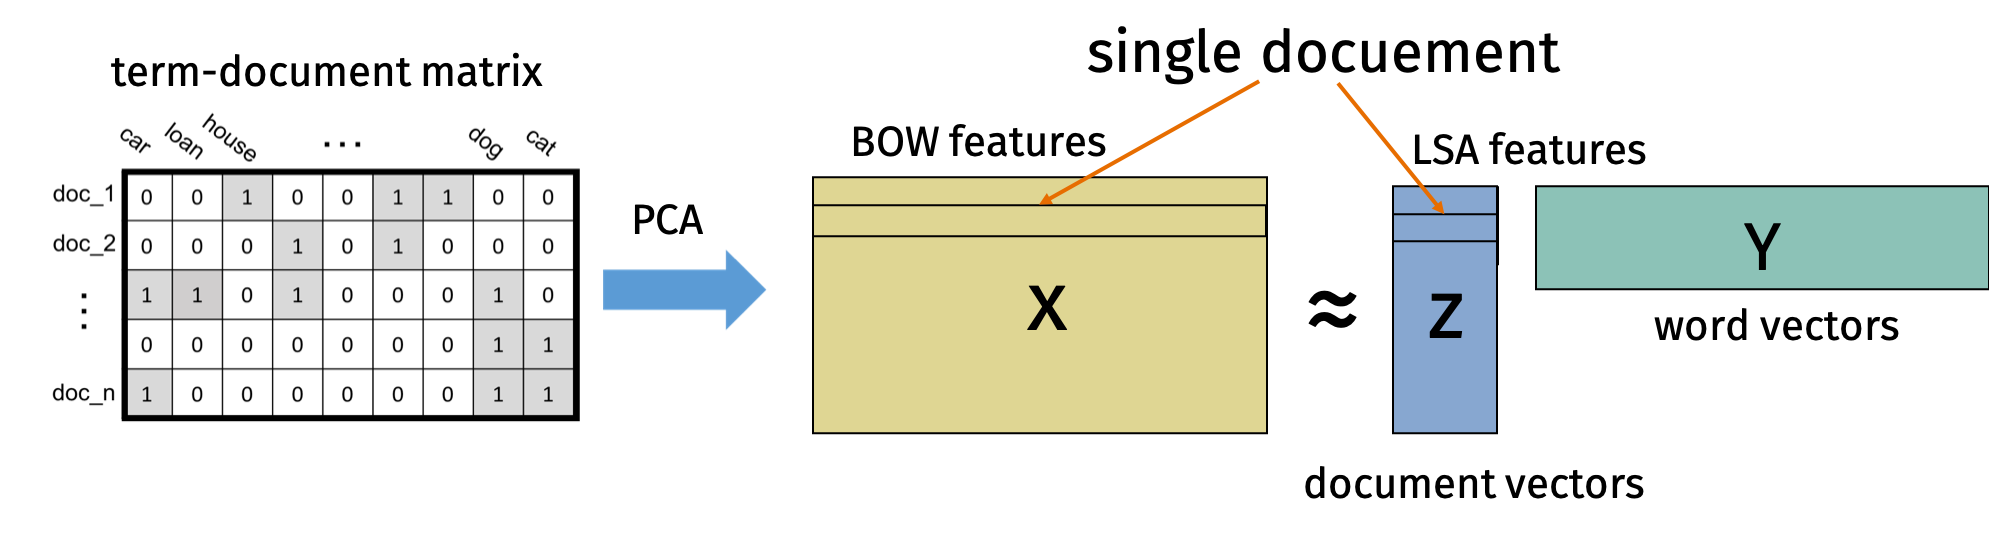
\includegraphics[width=\textwidth]{mylsa.png}
	\end{center}
	Each column of $\bv{z}$ corresponds to a latent ``category'' or ``topic''. 
	
	Similar documents have similar \emph{LSA document vectors}. I.e. $\langle \vec{z}_i, \vec{z}_j\rangle$ is large. Provide a more compact ``finger print'' for documents than the long \emph{bag-of-words vectors}. Useful for e.g search engines.  
\end{frame}

\begin{frame}
	\frametitle{latent semantic analysis}
	LSA vetors often provide a \emph{more meaningful} similarity metric than bag-of-words vectors. Capture high-level categorical information and eliminate document specific quirks. 
	\begin{center}
		Spectrum of data matrix $\bv{X}$. 
		
		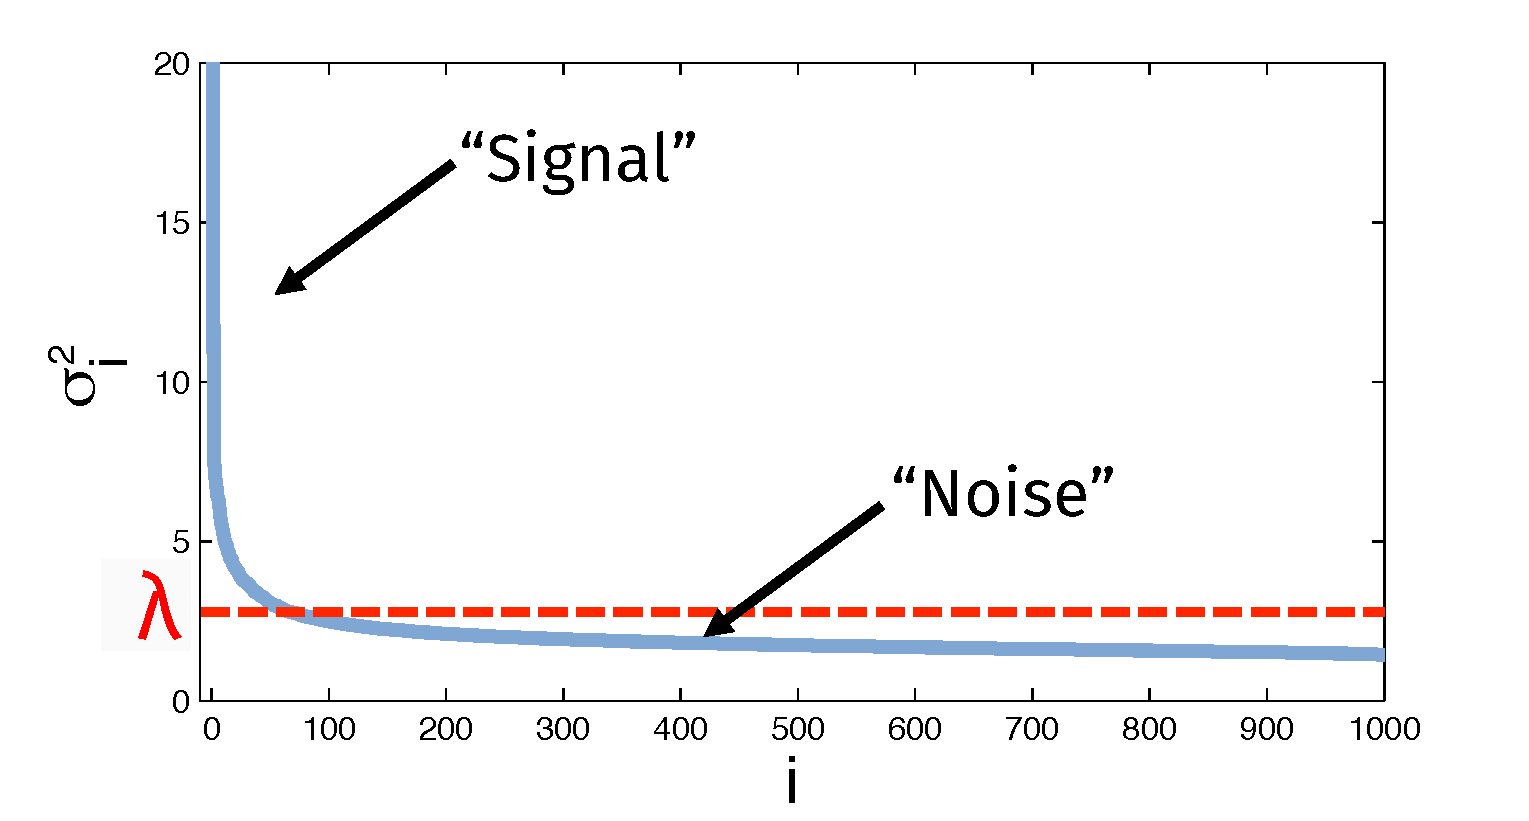
\includegraphics[width=.7\textwidth]{spectrumAnnotate.pdf}
	\end{center}
\end{frame}

\begin{frame}
	\frametitle{word embeddings}
	\begin{center}
		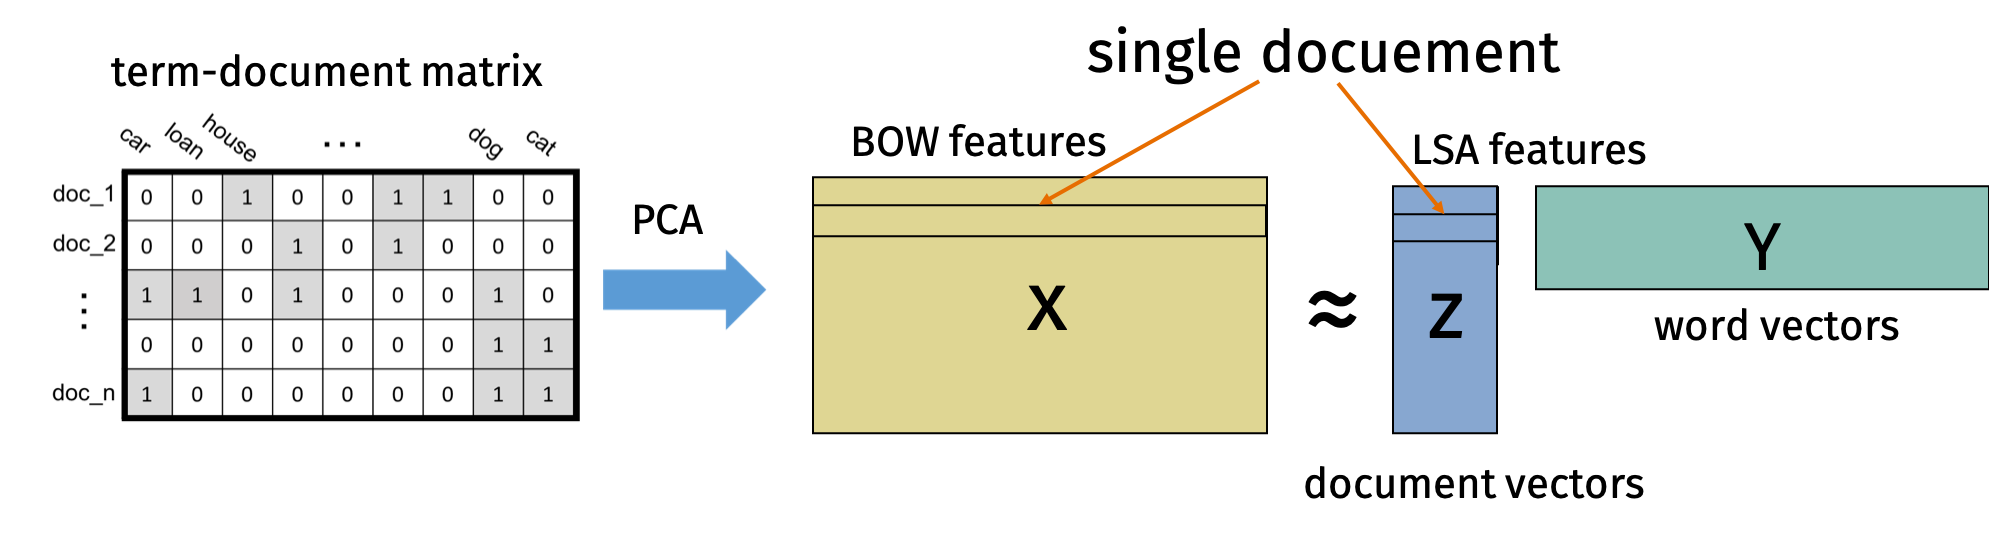
\includegraphics[width=.8\textwidth]{mylsa.png}
	\end{center}
	\begin{itemize}
		\item $\langle \vec y_i, \vec z_a \rangle \approx 1$ when $doc_i$ contains $word_a$. 
		\item If $doc_i$ and $doc_i$ both contain $word_a$, $\langle \vec y_i, \vec z_a \rangle \approx \langle \vec y_j, \vec z_a \rangle \approx 1$.
	\end{itemize}
	\vspace{-2em}
	\begin{center}
		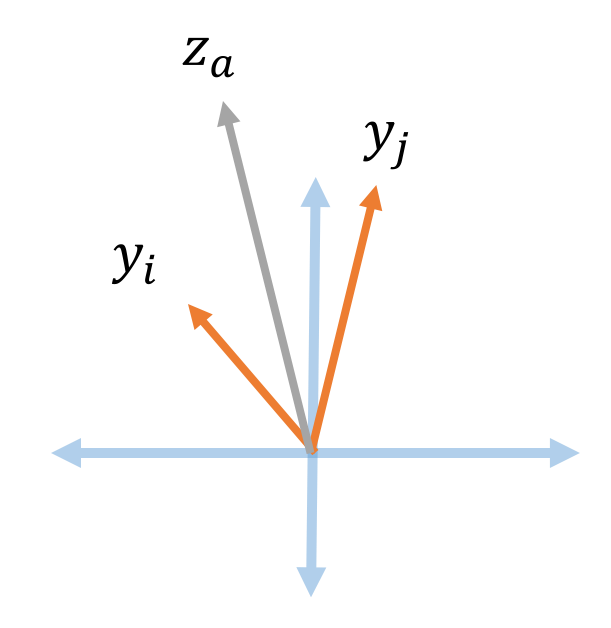
\includegraphics[width=.25\textwidth]{lsa2.png}
		
	If two words appear in the same document their, word vectors tend to point more in the same direction. 
	\end{center}
\end{frame}

\begin{frame}
	\frametitle{semantic embeddings}
	\textbf{Result:} Map words to numerical vectors in a \emph{semantically} meaningful way. Similar words map to similar vectors. Dissimilar words to dissimilar vectors.
	
	\begin{center}
		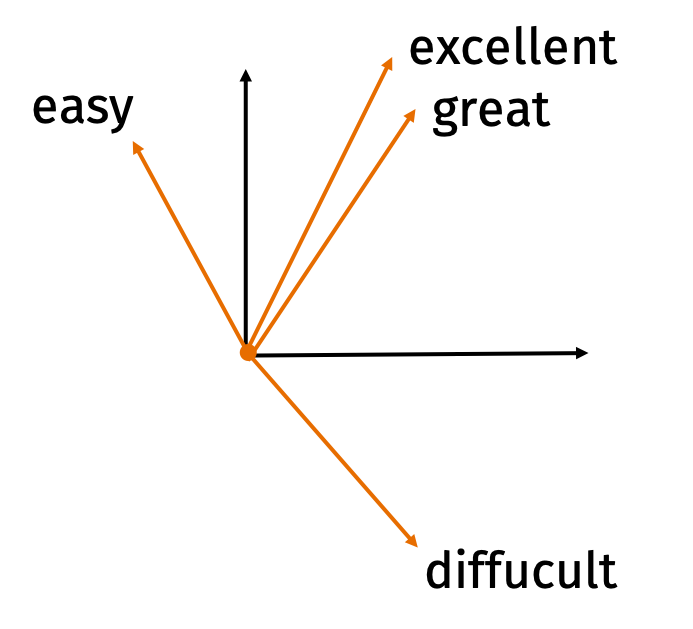
\includegraphics[width=.4\textwidth]{semantic_embedding.png}
		
		Extremely useful ``side-effect'' of LSA.
	\end{center}
\end{frame}


\begin{frame}
	\frametitle{word embeddings: motivating problem}
	
		\textbf{Review 1:} \textit{Very small and handy for traveling or camping. Excellent quality, operation, and appearance.}
		
		\textbf{Review 2:} \textit{So far this thing is great. Well designed, compact, and easy to use. I’ll never use another can opener.} 
	
		\textbf{Review 3:} \textit{Not entirely sure this was worth $\$20$. Mom couldn't figure out how to use it and it's fairly difficult to turn for someone with arthritis.}
	
	\begin{center}
		\textbf{\alert{Goal is to classify reviews as ``positive'' or ``negative''.}}
	\end{center}
\end{frame}


\begin{frame}
		\frametitle{bag-of-words features}
		\small
		\textbf{Vocabulary:} Small, handy, excellent, great, quality, compact, easy, difficult.
		
		\textbf{Review 1:} \textit{Very small and handy for traveling or camping. Excellent quality, operation, and appearance.}
		
		\begin{align*}
		\left[\hspace{2em},\hspace{2em},\hspace{2em},\hspace{2em},\hspace{2em},\hspace{2em},\hspace{2em},\hspace{2em}\right]
		\end{align*}
		
		\textbf{Review 2:} \textit{So far this thing is great. Well designed, compact, and easy to use. I’ll never use another can opener.} 
		\begin{align*}
		\left[\hspace{2em},\hspace{2em},\hspace{2em},\hspace{2em},\hspace{2em},\hspace{2em},\hspace{2em},\hspace{2em}\right]
		\end{align*}
		
		\textbf{Review 3:} \textit{Not entirely sure this was worth $\$20$. Mom couldn't figure out how to use it and it's fairly difficult to turn for someone with arthritis.}
				\begin{align*}
		\left[\hspace{2em},\hspace{2em},\hspace{2em},\hspace{2em},\hspace{2em},\hspace{2em},\hspace{2em},\hspace{2em}\right]
		\end{align*}
\end{frame}

\begin{frame}
	\frametitle{semantic embeddings}
	\small
	\begin{center}
		Bag-of-words approach typically only works for \emph{large data sets}. 
	\end{center}
	The features do not capture the fact that ``great'' and ``excellent'' are near synonyms. Or that ``difficult'' and ``easy'' are antonyms.
	
	\begin{center}
		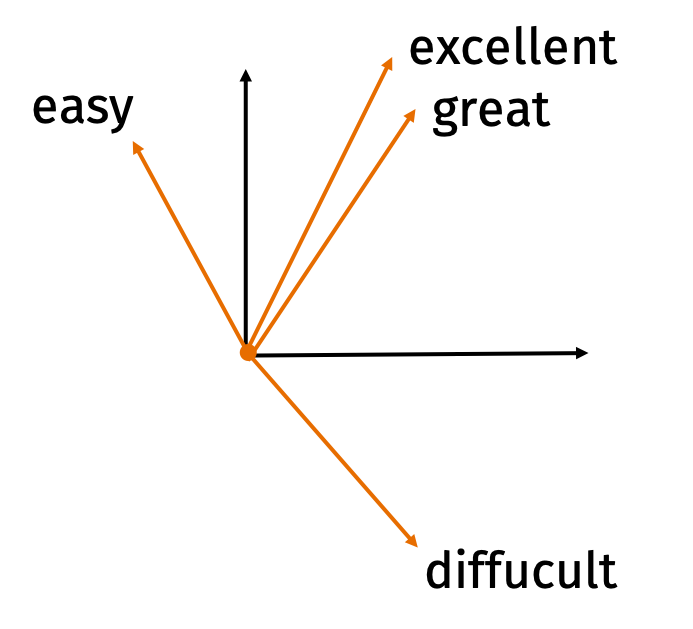
\includegraphics[width=.3\textwidth]{semantic_embedding.png}
	\end{center}
	This can be addressed by first mapping words to \emph{semantically meaningful vectors}. That mapping can be trained using a much large corpus of text than the data set you are working with (e.g. Wikipedia, Twitter, news data sets). 	
\end{frame}


\begin{frame}
	\frametitle{mdoern word embeddings}
	\textbf{Current state of the art models:} \texttt{GloVE}, \texttt{word2vec}.
	\begin{itemize}
		\item Based on same principal as LSA. 
		\item \texttt{word2vec} was originally presented as a shallow neural network model, but it can be viewed as a matrix factorization method (Levy, Goldberg 2014).
	\end{itemize}
\end{frame}


\begin{frame}
	\frametitle{word embeddings}
	\small
	Another view on word embeddings from LSA:
	\begin{center}
		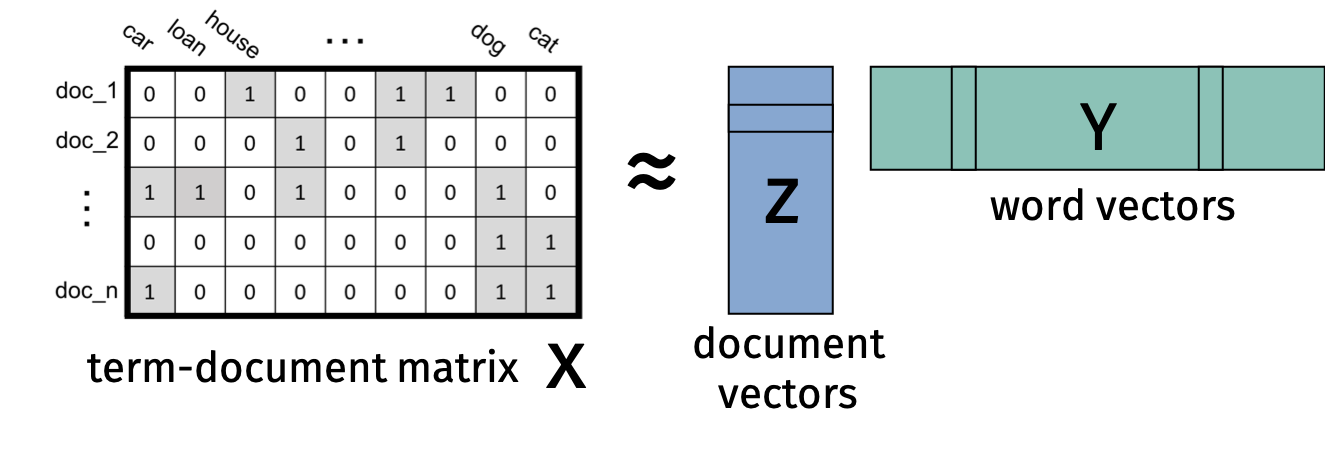
\includegraphics[width=.8\textwidth]{mylsa2.png}
	\end{center}
	Choose $\bv{Z}$ to have orthogonal columns. E.g. $\bv{Z} = \bv{U}_k$ and $\bv{Y} = \bs{\Sigma}_k\bv{V}_k^T$.
	\begin{itemize}
		\item $\bv{X} \approx \bv{Z}\bv{Y}$
		\item $\bv{X}^T\bv{X} \approx \bv{Y}^T\bv{Z}^T\bv{Z}\bv{Y} = \bv{Y}^T\bv{Y}$
		\item So for $word_i$ and $word_j$, $\langle \vec{y}_i, \vec{y}_j\rangle \approx [\bv{X}^T\bv{X}]_{i,j}$.   
	\end{itemize}
\vspace{-.5em}
	\begin{center}
		\large
	\alert{What does the $i,j$ entry of $\bv{X}^T\bv{X}$ reprent?}
\end{center}
\end{frame}

\begin{frame}
	\frametitle{word embeddings}
	\small
	$\langle \vec{y}_i, \vec{y}_j\rangle$ is \emph{larger} if $word_i$ and $word_j$ appear in more documents together (high value in \textbf{word-word co-occurrence matrix}. Similarity of word embedding vectors mirrors similarity of word context.
	
	\textbf{General word embedding recipe:}
	\begin{enumerate}
		\item Choose similarity metric $k(word_i,word_j)$ which can be computed for any pair of words. 
		\item Construct \emph{symmetric} similarity matrix $\bv{M} \in \R^{n\times n}$ with $\bv{M}_{i,j} = k(word_i,word_j)$. 
		\item Find \emph{symmetric} low rank factorization $\bv{M} \approx \bv{Y}^T\bv{Y}$ where $\bv{Y} \in \R^{k\times n}$. 
		\item Columns of $\bv{Y}$ are word embedding vectors. 
	\end{enumerate}
\end{frame}

\begin{frame}
	\frametitle{word embeddings}
	\small
	\begin{center}
		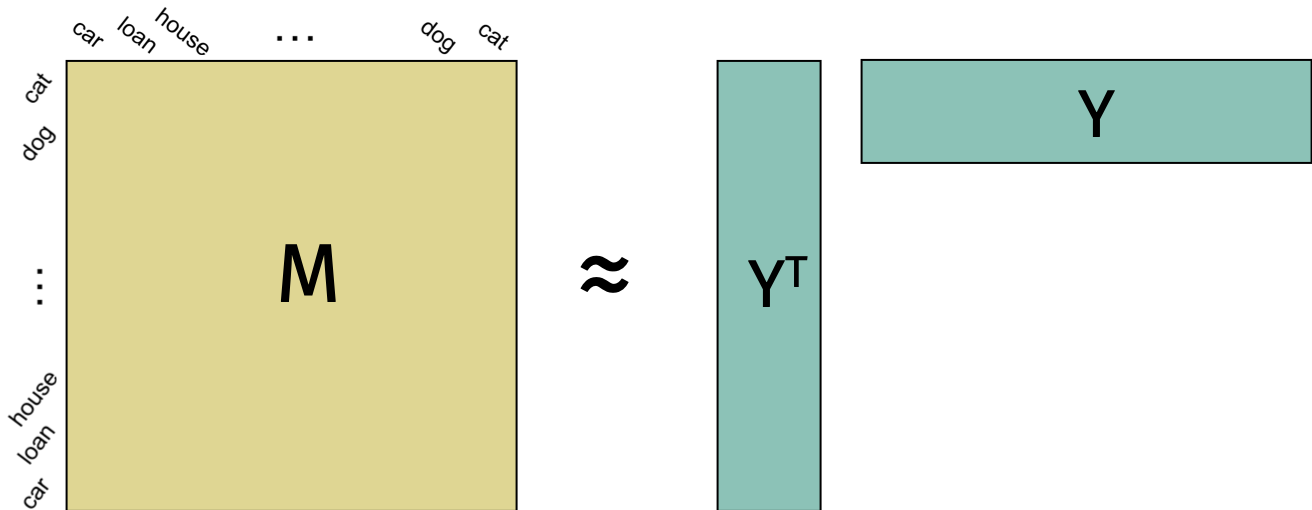
\includegraphics[width=.7\textwidth]{similarity_fact.png}
	\end{center}
	How do current state-of-the-art methods differ from LSA?
	\begin{itemize}
		\item Similarity based on co-occurrence in smaller chunks of words. E.g. in sentences or in any consecutive sequences of 10 words.
		\item Usually transformed in non-linear way. E.g. $k(word_i,word_j) = \frac{p(i,j)}{p(i)p(j)}$ where $p(i,j)$ is the frequency both $i,j$ appeared together, and $p(i)$, $p(j)$ is the frequency either one appeared. 
	\end{itemize}
	
\end{frame}

\begin{frame}
	\frametitle{easiest way to use word embeddings}
	If you want to use word embeddings for your project, the easiest approach is to download \emph{pre-trained} word vectors:
	\begin{itemize}
		\item \textbf{Original gloVe website:} \url{https://nlp.stanford.edu/projects/glove/}.
		\item \textbf{Compilation of many sources:} \url{https://github.com/3Top/word2vec-api}
	\end{itemize}
\end{frame}

\begin{frame}
	\frametitle{using word embeddings}
	How to go from word embeddings to features for a whole sentence or chunk of text?
	\begin{center}
	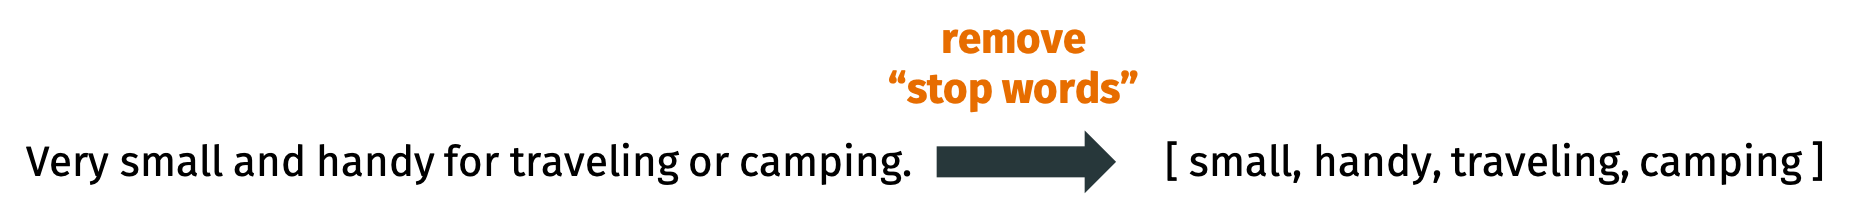
\includegraphics[width=1\textwidth]{step1.png}
	
	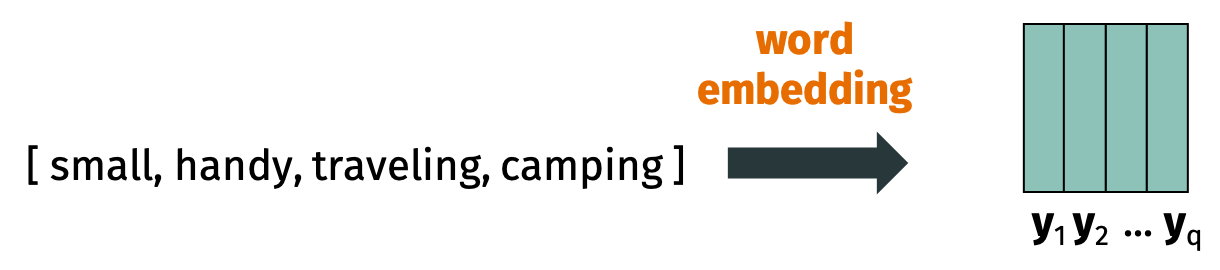
\includegraphics[width=.7\textwidth]{step2.png}
	
	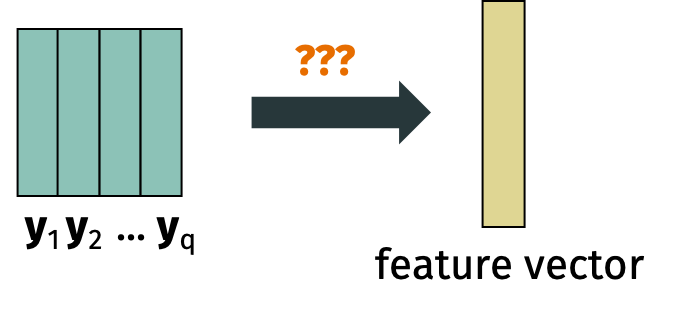
\includegraphics[width=.5\textwidth]{step3.png}
	\end{center}
\end{frame}

\begin{frame}
	\frametitle{using word embeddings}
	\textbf{A few simple options:} 
		\vspace{-.5em}
	
	Feature vector $\vec{x}= \frac{1}{q} \sum_{i=1}^q \vec{y}_q$. 
	\vspace{-1em}
	\begin{center}
		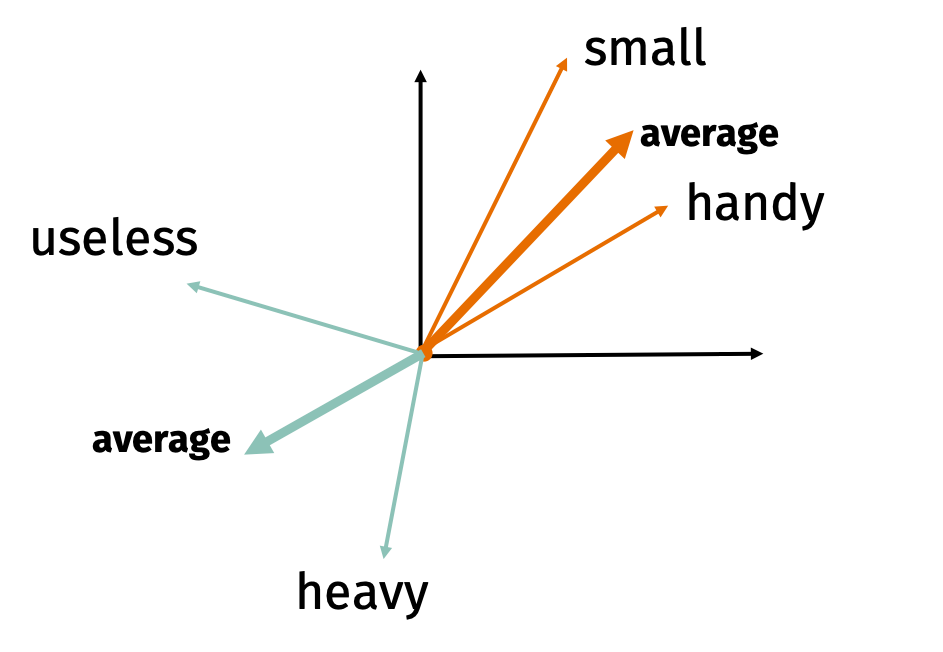
\includegraphics[width=.4\textwidth]{average_wordvec.png}
	\end{center}
	\vspace{-.5em}
	
	Feature vector $\vec{x}= [\vec{y}_1, \vec{y}_2, \ldots, \vec{y}_q]$. 
	\vspace{-1em}
	\begin{center}
		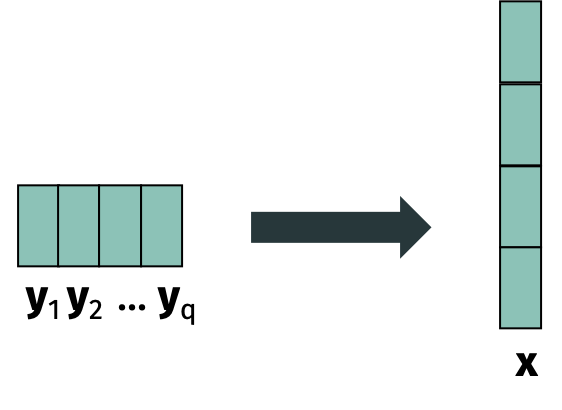
\includegraphics[width=.4\textwidth]{concat.png}
	\end{center}
\end{frame}

\begin{frame}
	\frametitle{using word embeddings}
	\textbf{Better option than concatenation}: 
	To avoid issues with inconsistent sentence length, word ordering, etc. try concatenating a fixed number of top \emph{principal components} of the matrix of word vectors:
	\begin{center}
		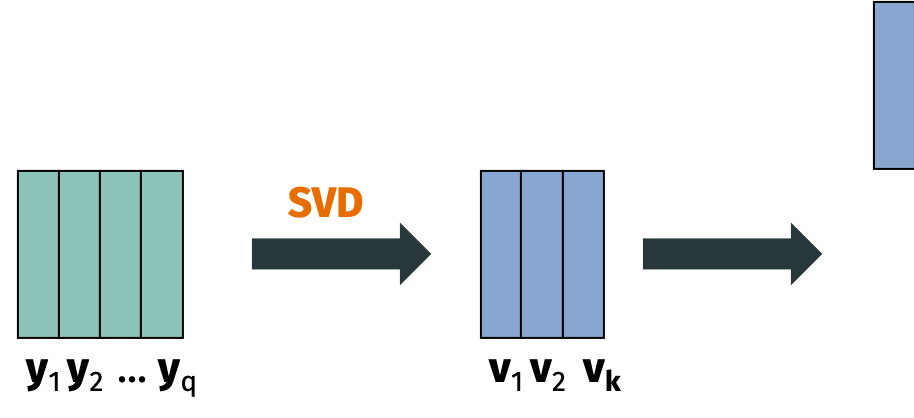
\includegraphics[width=.6\textwidth]{better_concat.png}
	\end{center}
\end{frame}
	
\begin{frame}
	\frametitle{data clustering}
	\textbf{Another important unsupervised learning task:} 
	\begin{center}
		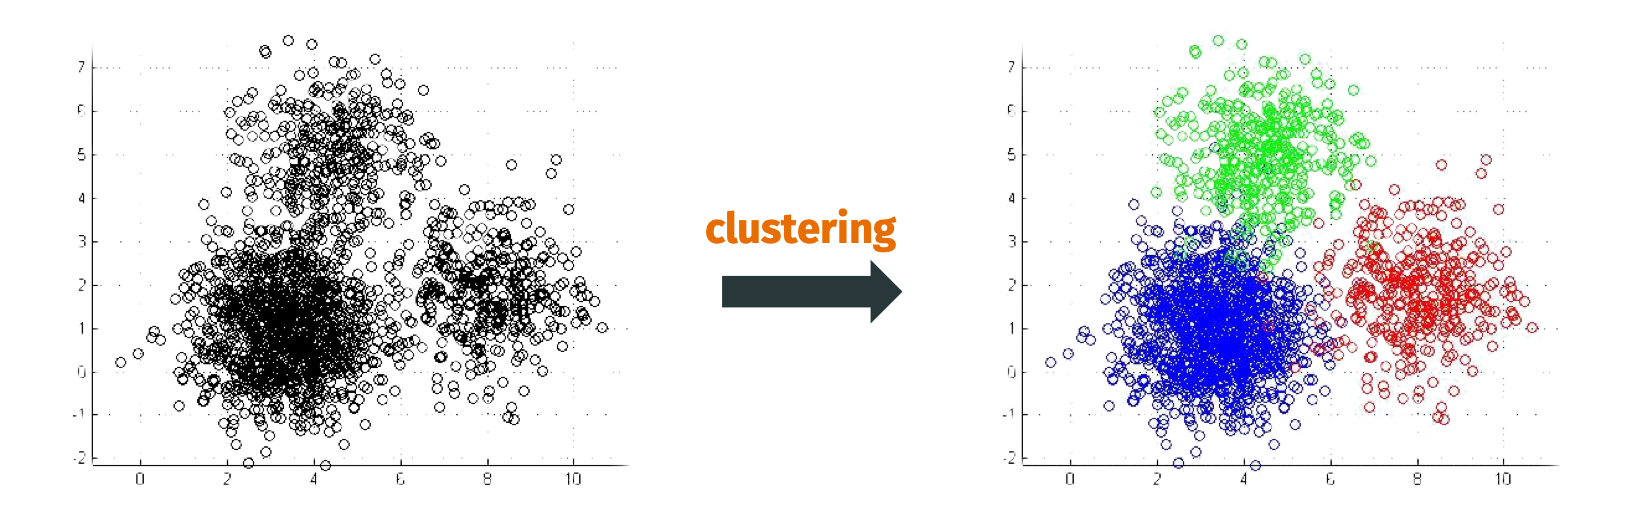
\includegraphics[width=\textwidth]{clustering_obj.png}
	\end{center}
Separate unlabeled data into natural clusters.
\begin{itemize}
	\item Exploratory data analysis. 
	\item Categorizing and grouping data. 
	\item Visualizing data. 
\end{itemize}
\end{frame}

\begin{frame}
	\frametitle{data clustering}
	\textbf{Example application:}
	\begin{center}
		\textbf{Images of Cats}.
		
		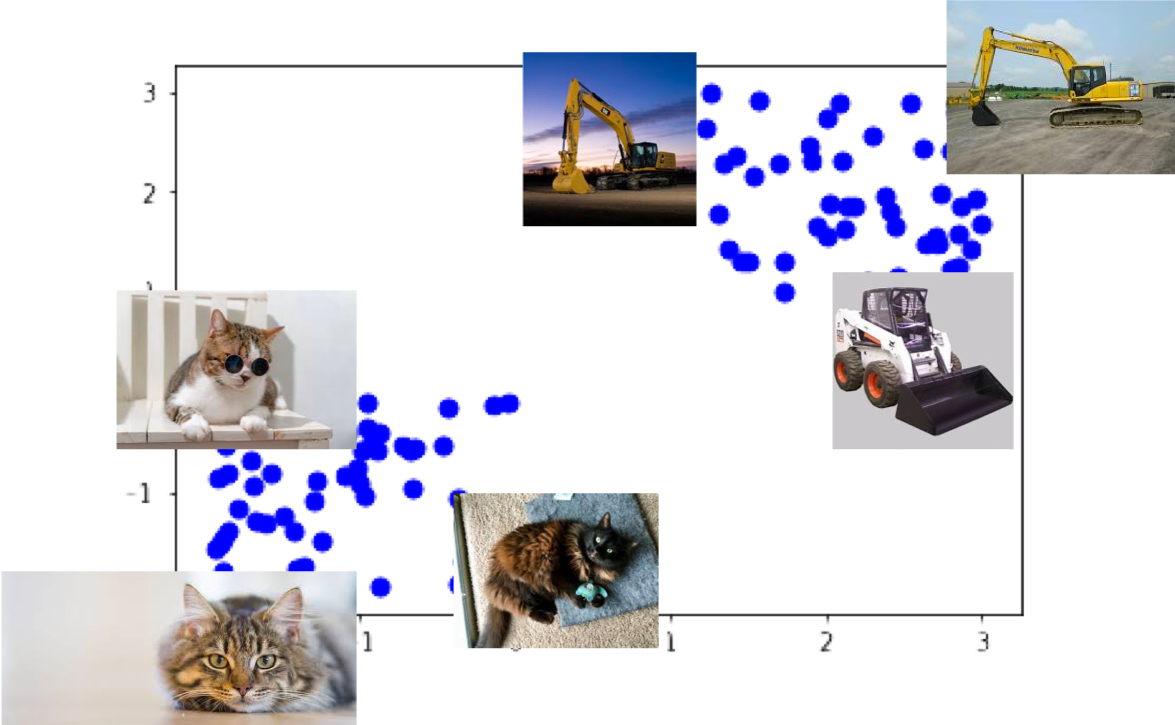
\includegraphics[width=.7\textwidth]{clustering_use.png}
	\end{center}
	Find sub-classes in your data which you may not have known about. Helps you decide how to adjust features or improve data set for a supervised application.
\end{frame}

\begin{frame}
	\frametitle{data clustering}
	\begin{center}
		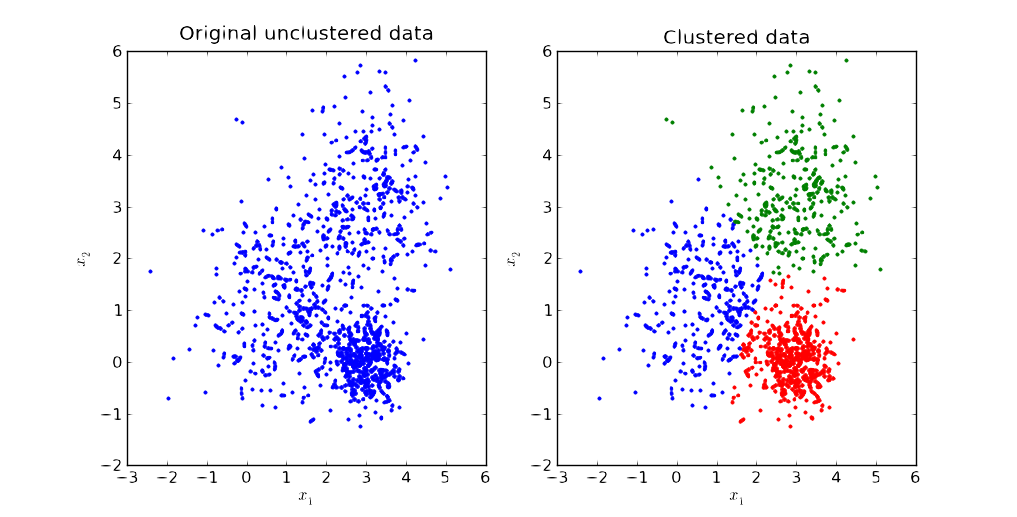
\includegraphics[width=.8\textwidth]{hardclustering.png}
	\end{center}
	\textbf{k-center clustering:}
	\begin{itemize}
		\item Choose centers $\vec{c}_1, \ldots, \vec{c}_k \in \R^d$. 
		\item Assign data point $\vec{x}$ to cluster $i$ if 
		$\vec{c}_i$ is the closest center to $\vec{x}$. 
	\end{itemize}
\end{frame}

\begin{frame}
	\frametitle{k-means clustering}
\end{frame}

\begin{frame}
	\frametitle{k-means clustering}
\end{frame}


\end{document} 



